\section{Co-working}
\indent Co-working je v samotnej podstate model poskytovania obchodných služieb, ktorý zahŕňa jednotlivcov, ktorí pracujú nezávisle alebo spolupracujú v spoločných kancelárskych priestoroch. Toto zdielanie jedných priestorov umožňuje tejto skupine ľudí zdieľať hodnoty, skúsenosti, nápady a profitovať zo synergického efektu, ktorý prináša sústredenie talentovaných pracovníkov na jednom mieste. Tiež umožňuje spoznávanie nových ľudí, ktorí môžu byť v budúcnosti pre človeka dôležití. Najčastejšími využívateľmi co-workingu sú napríklad obchodníci, umelci, programátori, konzultanti, dizajnéri, makléri, agenti, študenti, malé a začínajúce firmy \cite{co_working,co_working_2,co_working_3,co_working_4}.

\begin{figure}[H]
    \centering
    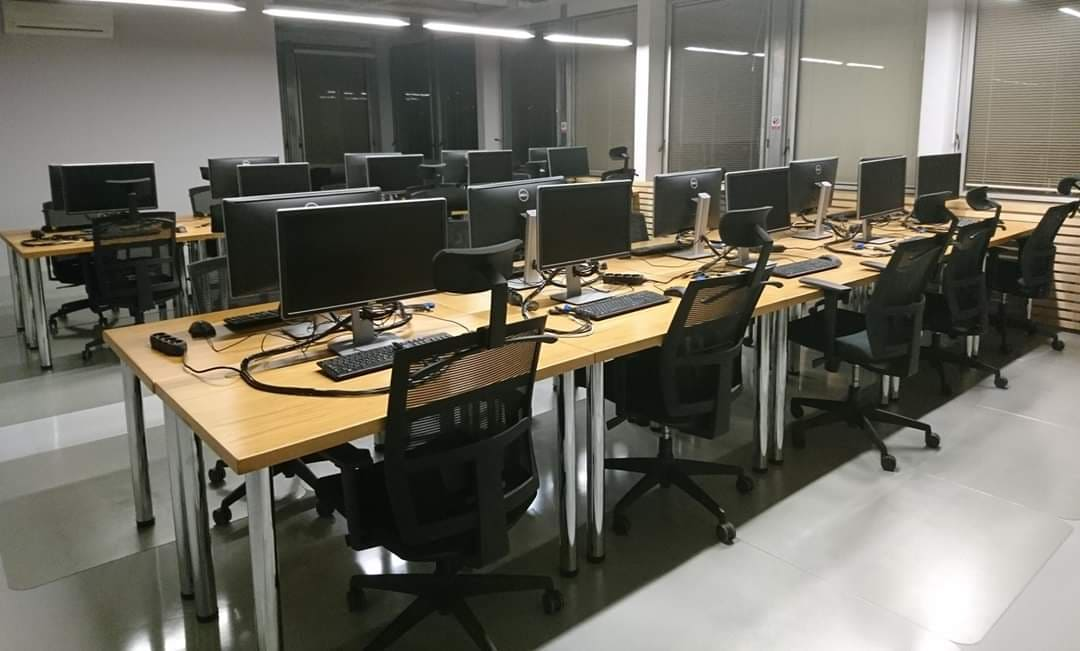
\includegraphics[scale=0.40]{img/ybase.jpg}
    \caption{Y-base študentský co-working space na internáte STU ŠD Mladosť Bratislava}
    \label{fig:img-ybase}
\end{figure}

\indent Pre účely co-workingu sa po celom svete začali budovať tzv. co-working centrá, ktorých počet každým rokom rastie. Vznik týchto centier je výsledkom hľadania stratégií, ako sa vyrovnať s rizikami a problémami nových, flexibilných štýlov práce. Veľa centier bolo založených internetovými podnikateľmi, ktorí chceli nájsť alternatívu k práci z kaviarní alebo k izolácii spôsobenej prácou z domu. Tieto centrá sú zväčša ihneď pripravené a vybavené potrebnými vecami k práci ako sú stoly, stoličky, tabule na písanie, kuchynka, internetové pripojenie, meetingové priestory, prípadne aj sieťová tlačiareň. To znamená, že pre bežného používateľa nevyžaduje začatie práce v takomto centre žiadne počiatočné alebo investičné náklady. Jediným poplatkom je zaplatenie členstva v centre \cite{co_working,co_working_2,co_working_3,co_working_4}. 

\subsection{História co-workingu}
\indent Slovo co-working v zmysle popisu ľudí, ktorí pracujú v akomkoľvek prostredí prvý krát, použila Bernie DeKoven v roku 1995. K prvému vzniku co-workingového priestoru, respektíve centra prišlo ale až v roku 2006 v San Franciscu pod vedením Brada Neuberga. Toto centrum sa nazývalo \textit{San Francisco Coworking Space} a bolo otvorené len 2 dni v týždni. Kuriozitou je, že prvý mesiac ho nikto nevyužíval, lebo hoci termín co-working bol známy, ale nikto ho nepočul pod významom ako co-working miesto alebo centrum \cite{co_working_spaces}. 

\begin{figure}[H]
    \centering
    
\includegraphics[scale=0.50]{img/coworking_space.jpg}
    \caption{Co-working centrum v San Franciscu \cite{co_working_spaces}}
    \label{fig:img-co-space}
\end{figure}

\indent Dnes sa vytváranie co-workingových centier pokladá za globálny fenomén, ktorý v niektorých mestách dosahuje ročný nárast až 24,2\%. Predpokladom je, že do roku 2022 bude celosvetovo vytvorených vyše 30500 centier alebo priestorov a viac ako 5,1 milióna členov. Co-working je nová cesta trvalo udržiavateľného spájania pracovného a osobného života. Je to globálny pilier, ktorý bude formovať spôsob našej práce v budúcnosti \cite{co_working_spaces}. 

\section{Co-working aplikácie}
\indent Co-working aplikácie sú aplikácie, ktoré slúžia na komunikáciu a manažovanie tímu pri práci viac ľudí na dosiahnutí určitého cieľa alebo výsledku. Týchto aplikácii na trhu existuje veľa, pričom niektoré sú bezplatné, niektoré sú platené a niektoré sú vyvinuté priamo vo firme, kde sa používajú a nemá k nim teda prístup nikto okrem danej firmy. Medzi najznámejšie patrí napríklad Slack, Facebook workplace, Trello, Microsoft Teams a iné.
 
\indent Tieto aplikácie majú slúžiť ako náhrada za co-workingové centrum v online svete. Keď si zoberieme služby, ktoré ponúkajú co-workingové centrá, tak sa dajú prirovnať k niektorým službám, ktoré ponúkajú aplikácie. Či už sa jedná o meetingové miestosti - v aplikácii sú to online chatové miestnosti v rámci tímu alebo o možnosť spoznávania nových ľudí osobne - v aplikácii online. 

\subsection{Slack}
\indent Slack je komunikačný nástroj vyvinutý pre pracovné využitie spoločnosťou Slack Technologies – „jedno miesto pre posielanie správ, nástroje a súbory“. To znamená, že Slack je softvér na posielanie „okamžitých“ správ s možnosťou pridania ďalších doplnkov podľa potreby používateľa. Tieto doplnky, ale nie sú potrebné na plynulý chod aplikácie pretože základnou funkciou Slacku je len posielanie správ. Na Slacku existujú 2 spôsoby komunikácie: 1. spôsob sú tzv. kanály, čo je v podstate skupinový rozhovor a 2. spôsob sú priame správy medzi dvoma používateľmi \cite{slack}. 

\subsubsection{História}
\indent Slack začal ako aplikácia na internú komunikáciu v spoločnosti Stewarda Butterfielda Tiny Speck pri vývoji online hry Glitch – hra bola vydaná v septembri 2011. Pre širšiu verejnosť bol Slack vydaný v auguste 2013. Slack je skratka pre: „Searchable Log of All Conversation and Knowledge“, čo vo voľnom preklade znamená: „Protokol prehľadávania všetkých konverzácií a znalostí.“

\indent V marci 2015 spoločnosť Slack oznámila, že bola vo februári 2015 opakovane napadnutá hackermi počas 4 dní. Počas tohto útoku boli ohrozené údaje používateľov. Medzi tieto údaje patrili e-mailové adresy, používateľské mená, heslá, telefónne čísla a Skype mená, ktoré boli priradené k ich účtom. Po tomto útoku Slack pridal do svojej aplikácie dvojfaktorovú autentifikáciu \cite{slack}. 

\subsubsection{Používateľské rozhranie}
\indent Keď chce používateľ začať používať Slack, musí najskôr cez stránku Slacku vytvoriť názov svojej „inštancie“ Slacku. Tento názov sa potom stane súčasťou URL adresy, ktorá slúži ako pozvánka. Potom buď cez stránku Slacku alebo poslaním URL pozve ľudí, ktorých chce mať na svojom Slacku. 

\indent Po akceptovaní tejto pozvánky si používateľ vytvorí účet. Po prihlásení pod týmto účtom sa používateľovi otvorí stránka „inštancie“ Slacku alebo ak má nainštalovanú aplikáciu, tak aplikácia Slacku viď. Obr.~\ref{fig:img-slack-app}

\indent Kanály na Slacku môžu byť verejné, čo znamená, že každý člen skupiny ho vidí a môže sa k nemu pripojiť alebo súkromné, čo znamená, že ich vidia len ľudia pridaní alebo pozvaní. Priame správy sú vždy súkromné, ale môžu obsahovať až 8 ľudí.

\begin{figure}[H]
    \centering
    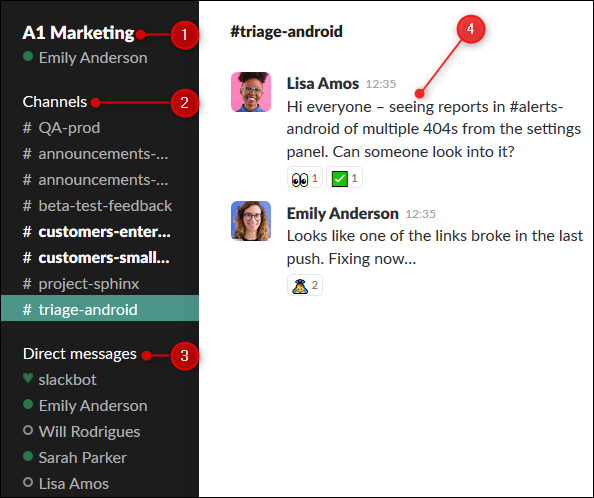
\includegraphics[scale=0.80]{img/obr1.png}
    \caption{Slack aplikácia \cite{slack}}
    \label{fig:img-slack-app}
\end{figure}
\begin{enumerate}
    \item Názov skupiny/inštancie
    \item Zoznam kanálov 
    \item Zoznam kontaktov
    \item Okno chatu
\end{enumerate}


\subsubsection{Doplnky}
\indent Do aplikácie Slack je možné pridať rôzne doplnky, či už priamo vytvorené firmou Slack Technologies alebo inými firmami ako je Google, Jira, Trello a iné. Celkový prehľad doplnkov Slack uvádza na svojej stránke, kde sa vie používateľ priamo prekliknúť aj na stránku daného doplnku, kde je napísané čo doplnok prináša do Slacku, plus tutoriál ako ho používať a prípadne video používania doplnku. Doplnok je možné pridať priamo cez aplikácie Slack alebo cez stránku Slacku.

\indent Doplnky sú na stránke rozdelené do kategórií, do ktorých viac menej patria. Tieto kategórie sú rôzne od botov, ktorí automaticky ako je niečo zmenené na strane doplnkovej aplikácie, pridajú do daného kanála upozornenie alebo správu, až po priame importy, ktoré pridávajú funkcionalitu priamo do Slacku.
\subsubsection{Výber najznámejších importov}
\begin{itemize}
    \item Google Drive
    \item Google kalendár
    \item Trello
    \item Twitter
    \item Outlook kalendár
    \item OneDrive
    \item GitHub
    \item Polly (hlasovania a prieskumy)
    \item Jira Cloud
    \item TimeBot
    \item WorkBot
    \item Giphy
    \item Doodle Bot
\end{itemize}
\subsubsection{Cena}
\indent Slack ako taký je zadarmo, ale sú tam isté obmedzenia. Hlavným obmedzením je prístup len k 10000 najnovším správam a používateľ môže pridať len 10 doplnkov na inštanciu. Ďalšími obmedzeniami sú napríklad žiadni jedno-kanálový alebo viac-kanálový hostia a limitované možnosti administrácie. 

\indent Ak chce používateľ sprístupniť celú funkcionalitu, tak je to dosť drahé. Vychádza to približne 12 dolárov na používateľa mesačne pri ročnej platbe alebo približne 15 dolárov pri mesačnej platbe. Ak teda napríklad máme 1000 člennú skupinu, ktorá chce používať Slack, vychádza to približne 144000 dolárov pri ročnej platbe \cite{slack}.

\subsection{Facebook Workplace}
\indent Čas, ktorý ľudia strávili v práci chatovaním, prezeraním a likovaním príspevkov na Facebooku, znižoval produktivitu ľudí v hodnote cca 3,5 bilióna dolárov. Táto téma sa pretriasala cez seriózne diskusie, až po vytváranie vtipných obrázkov. Preto sa ľudia v spoločnosti Facebook začali zaoberať touto otázkou, či sa funkcionalita Facebooku nedá preniesť aj na pracovnú aplikáciu. Toto dalo počiatok Facebook Workplacu, ktorý podľa slov jeho stvoriteľov má podporiť kolaboráciu tým, že ju urobí zábavnou a jednoduchšou pre ľudí \cite{facebook_workplace,facebook_workplace_2}.

\begin{figure}[H]
    \centering
    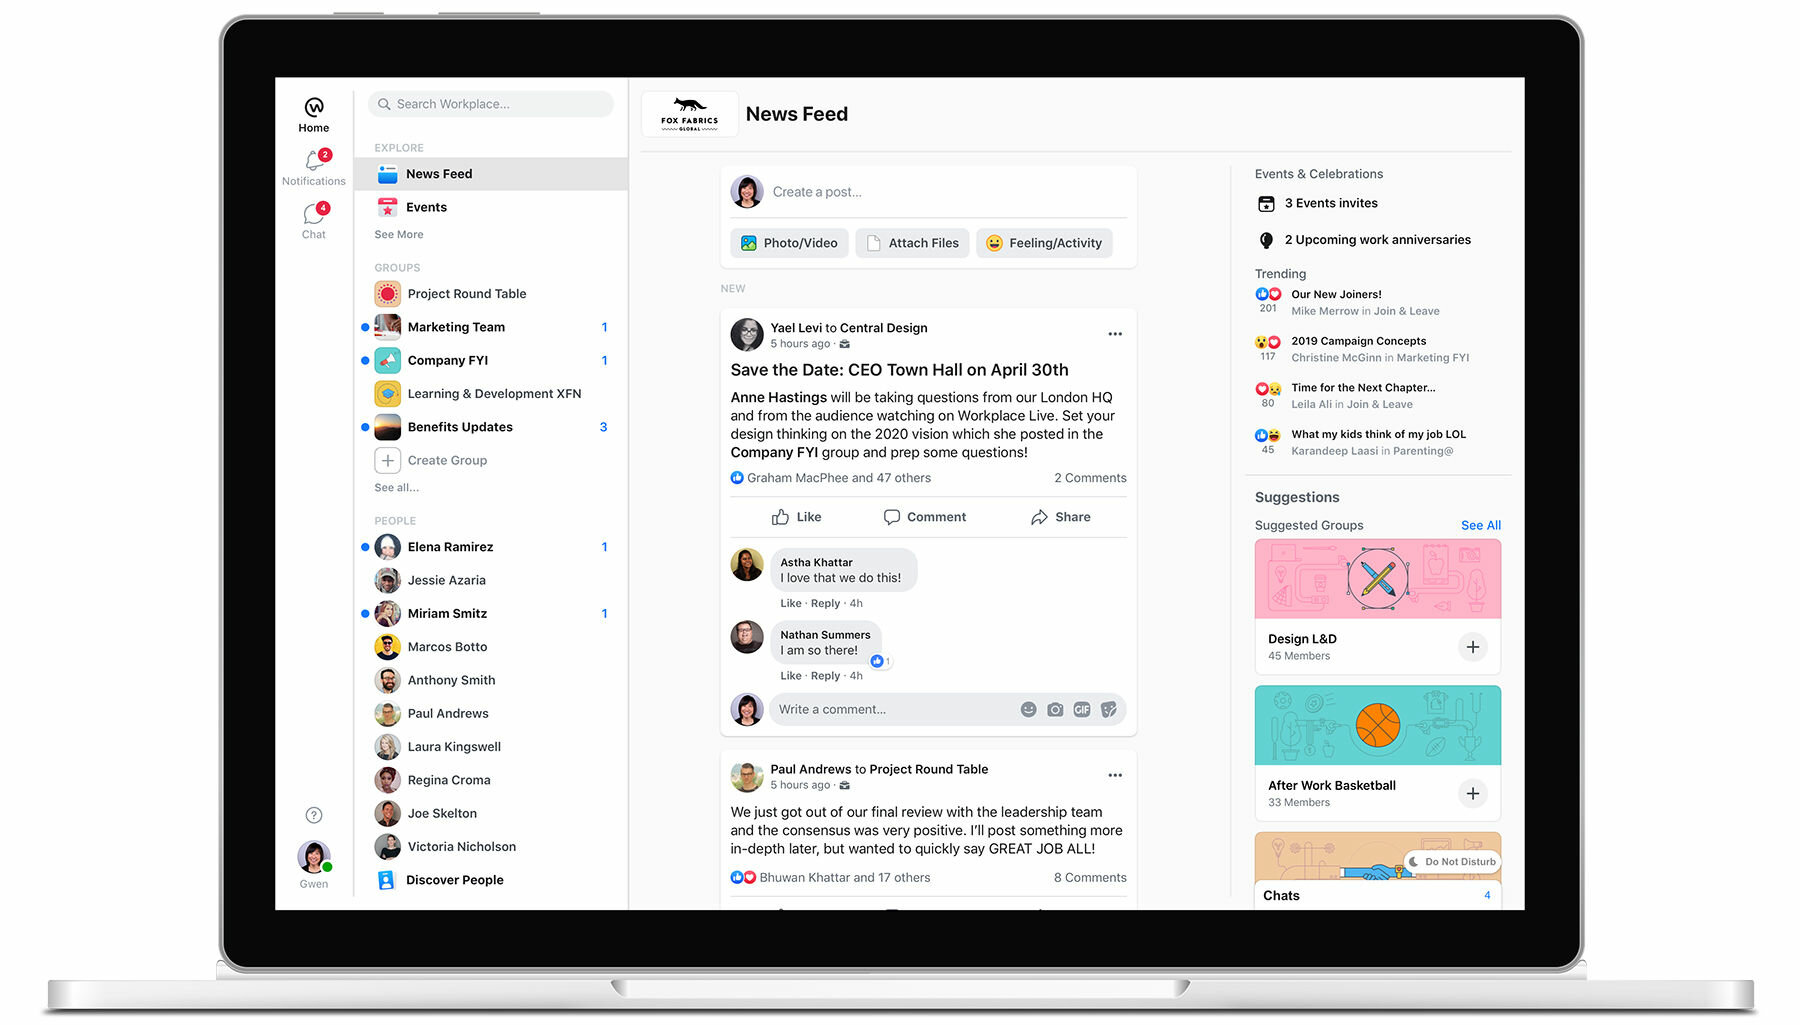
\includegraphics[scale=0.25]{img/obr-fb-workplace.jpg}
    \caption{Stránka Facebook Workplace \cite{facebook_workplace_2}}
    \label{fig:img-fb-workplace}
\end{figure}

\subsubsection{História}
\indent Myšlienka sa začala rozvíjať v roku 2014, keď prišla myšlienka nasmerovať tendenciu členov tímu prechádzať Facebook počas pracovnej doby k lepšej produktivite a spolupráci. Začiatkom roku 2015 sa začala do vybraných spoločností zavádzať beta verzia s názvom Facebook at Work. Keďže Facebook týmto vstupoval do neznámych vôd, bolo samozrejmé, že beta verzia sa veľmi často menila. V polovici roka 2015 Facebook získal veľmi silného spojenca pre vývoj tejto aplikácie - The Royal Bank of Scotland – Škótska národná banka. Tá presadila masívne využitie tejto beta verzie Facebook at Work, kedy sa vytvorilo až 100000 nových účtov. 

\indent Ku koncu roka 2015 mal Facebook veľa kladných ohlasov na túto svoju vyvíjanú platformu od manažérov firiem, kde bol Facebook at Work zavedený. Bolo to hlavne zapríčinené tím, že zamestnanci mali veľmi jednoduchý prístup k pracovným profilom svojich kolegov a podriadených. Tak isto kvôli prehľadnosti sa názov zmenil na Facebook Workplace.

\indent  V októbri 2016 boli oficiálne na trh uvedené pracovné a mobilné verzie aplikácie Facebook Workplace. Týmto Facebook začal konkurovať gigantom ako Slack a Microsoft Teams na poli podnikového softvéru \cite{facebook_workplace,facebook_workplace_2}.
\subsubsection{Používateľské rozhranie}
\indent Rozhranie Workplacu je podľa slov používateľov na 95\% rovnaké ako na Facebooku. Väčšina populárnych funkcií Facebooku bola pridaná tiež do Workplacu:
\begin{itemize}
    \item Newsfeed – zobrazujú sa tu všetky tímové aktivity ako napríklad príspevky členov tímu, firemné akcie a všetky informácie týkajúce sa práce prihláseného používateľa
    \item Live tools – funkcie na živý prenos (Live streaming)
    \item Skupiny – manažéri môžu vytvárať skupiny na pracovisku a tým udržiavať aktivity jednotlivých skupín/tímov na jednom  mieste
    \item Správy – používatelia si môžu písať so svojimi kolegami
\end{itemize}

\indent Pre používateľov je toto síce výhoda, keďže sa nemuseli učiť používať nový nástroj, avšak pre firmy je problém prijať v podstate napodobeninu Facebooku ako pracovnú aplikáciu. Kvôli tomuto Facebook aj oddelil profily Facebooku a Workplacu, nakoľko donedávna boli tieto profily prepojené a aj vytváranie účtu sa robilo cez profil Facebooku. 
\subsubsection{Cena}
\indent Workplace je pre firmy na prvé tri mesiace zadarmo. Potom sa jeho cena odvíja od počtu aktívnych účtov prípadne existuje bezplatná verzia so základnými vlastnosťami. Do 1000 používateľov sa platia 3 doláre za každého, do 10000 používateľov sa platí 2 doláre za každého a nad 10000 používateľov sa platí 1 dolár za každého.  Pre neziskové organizácie a akademické účely je úplne zadarmo aj po 3 mesiacoch \cite{facebook_workplace,facebook_workplace_2}.

\subsection{Microsoft Teams}
\indent Microsoft Teams je aplikácia na pracovnú komunikáciu a kolaboráciu od spoločnosti Microsoft, ktorá bola vyvinutá, aby konkurovala aplikáciám Slack, Workplace, HipChat. Vo svojej najjednoduchšej podobe je to aplikácia umožňujúca komunikáciu medzi členmi vytvorenej skupiny na báze miestností - kanálov. Microsoft sa už pred vydaním Teams pokúšal presadiť na trhu pracovných aplikácií pomocou svojho Skype for Business. Táto aplikácia však nenaplnila očakávania tak, ako jej lepšia verzia Teams \cite{ms_teams}. 
\subsubsection{História}
\indent V marci 2016 chcel Microsoft kúpiť Slack za 8 miliárd dolárov avšak Bill Gates bol proti a skôr presadzoval zlepšenie ich aplikácie Skype for Business. Tento nákup presadzoval hlavne vysoko postavený pracovník Microsoftu Qi Lu. Ten ale ešte v roku 2016 opustil spoločnosť a v novembri toho istého roku Microsoft oznámil prácu na aplikácii Teams, ako na aplikácii, ktorá má konkurovať Slacku. 

\indent Slack uznal Teams ako konkurenčnú službu avšak uviedol, že nekonkurujú rovnakému publiku, nakoľko Teams v tej dobe neumožňoval ľudom bez predplateného balíka Office 365 vstup do aplikácie Teams. Slack to zdôvodňoval aj tým, že neprepokladá sa, že by malé a stredné podniky využívajúce Slack, začali používať platenú službu Office, ktorej Teams bol súčasťou. Neskôr však Teams rozšíril o možnosť pridania nových ľudí aj bez predplateného balíka Office 365. Slack na toto reagoval integráciou služieb od Google (Drive, Kalendár, Gmail). 

\indent V roku 2017 sa udiali 2 udalosti. Prvou bolo, že Teams nahradili MS Classroom v balíku Office 365 for Education. Druhou udalosťou bola správa v septembri, že Teams nahradzujú Skype for Business. Tým bola aj ukončená služba Skype for Business. 

\begin{figure}[H]
    \centering
    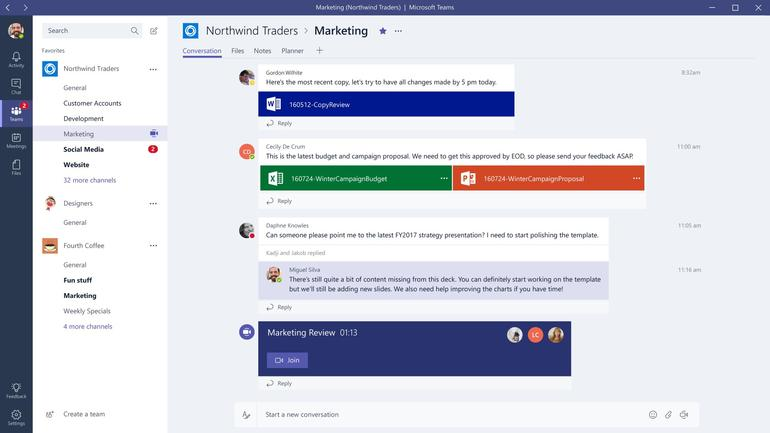
\includegraphics[scale=0.70]{img/obr-ms-teams.jpg}
    \caption{Aplikácia MS Teams \cite{ms_teams_2}}
    \label{fig:img-ms-teams}
\end{figure}

\indent V júli 2018 oznámil Microsoft bezplatnú verziu služby Teams s obmedzeniami typu počet používateľov a kapacitu ukladania súborov. V novembri 2019 dosiahol Teams 20 miliónov používateľov, čo bol nárast o 7 miliónov od júla 2019 \cite{ms_teams}. 
\subsubsection{Používateľské rozhranie}
\indent Rozhranie Teams je veľmi podobné tomu na Slacku. Na vytvorenie tímu treba vytvoriť URL, ktorá potom slúži rovnako ako na Slacku na pozývanie používateľov. Po prihlásení sa pomocou Microsoft účtu, môžu potom jednotliví používatelia vytvárať miestnosti, do ktorých môžu pridávať príspevky. Tak isto je možná komunikácia medzi používateľmi bez miestnosti štýlom, ako je v aplikácii Skype. Tu je povolená hlasová aj video komunikácia Skype štýlom. 

\indent Mimo klasických miestností-kanálov je možne vytváranie aj takzvaných meeting miestností, ktoré slúžia na komunikáciu počas pracovných porád, meetingov a stretnutí. Tieto miestnosti umožňujú priame pridanie času a dátumu meetingu do kalendára Outlooku. Na náhľade nástenky po otvorení miestnosti je možné vidieť, v akom stave stretnutie je: ešte nezačalo, prebieha, ukončené. 

\indent Microsoft do Teams pridal aj funkciu podobnú funkcionalite Trella – dashboard. Pomocou tejto funkcie môžu manažéri, učitelia, vedúci pracovníci prideľovať a sledovať prácu používateľov. Tak isto sa jednotlivé úlohy na tejto „nástenke úloh“ dajú komentovať, presúvať alebo hodnotiť.

\indent Samozrejmosťou je veľmi dobrá kompatibilita s inými aplikáciami Microsoftu ako je Word, Excel, PowerPoint, OneDrive. Jednotlivé dokumenty týchto aplikácii sa dajú priamo posielať, upravovať v aplikácii Teams a tak majú jednotliví používatelia vždy najaktuálnejšiu verziu dokumentu k dispozícii. Microsoft pridal aj komunikáciu s aplikáciami od iných vývojárov, ako je GitHub, Evernote, Zendesk pomocou konektorov. Táto komunikácia slúži najmä na posielanie upozornení, že na strane druhej aplikácii prišlo k nejakej zmene – napríklad príde upozornenie do miestnosti, že niektorý používateľ pushol na git niečo nové \cite{ms_teams}.  
\subsubsection{Doplnky}
\indent Do Teams podobne ako do Slacku je možné pridanie rôznych doplnkov od iných vývojárov. Tieto doplnky sú však po väčšine len Boti, ktorých úlohou je posielanie upozornení, že na strane druhej aplikácie prišlo k nejakej zmene – pridanie nových vecí na GitHub, zmena v Evernote a iné. Týchto Botov je potvrdených zatiaľ 85 a 70 konektorov – aplikácie, ktoré slúžia nielen na posielanie upozornení. 
\subsubsection{Cena}
\indent Microsoft Teams je v svojej jednoduchšej podobe zadarmo. Obmedzeniami bezplatnej verzie sú napríklad prístup na OneDrive, plánovania schôdze, nahrávanie schôdze pomocou Microsoft Stream, technická podpora, viacfaktorová autentifikácia pre všetkých používateľov. 

\indent Platených verzii je viac. Tieto verzie sú viazané na balík Office 365, ktorý má používateľ/firma zaplatený. Za balík Office 365 Business Essentials pýta Microsoft 4,20€ za používateľa, mesačne, s ročnou viazanosťou a za balík Office 365 Business Premium 10,50€ za používateľa, mesačne, s viazanosťou na rok. V balíku Premium je zahrnutá kompletná funkcionalita aplikácie Teams. Pri balíčku Essentials sú tam stále isté obmedzenia \cite{ms_teams}.

\subsection{Trello}
\indent Trello je aplikácia na vytváranie pracovnej nástenky v kanbanskom štýle. Aplikácia od roku 2017 patrí spoločnosti Atlassian, avšak vydaná bola v roku 2011 spoločnosťou Fog Creek Sowtvare. Aplikácia obsahuje virtuálnu nástenku, kde členovia tímu môžu vytvárať, organizovať a priraďovať úlohy v rámci projektu. Použitý kanbanský/kartový štýl umožňuje členom tímu vzájomne spolupracovať a komunikovať pri práci na projekte. Používatelia môžu k projektovým kartám pridávať komentáre, odkazy, súbory a fotografie. Trello existuje v rôznych podobách. Existuje webová aplikácia, desktopová aplikácia, či už pre Windows alebo MacOS a tak isto existujú aj mobilné aplikácie pre Android a iOS. Existuje aj import aplikácie do Slacku \cite{trello}.
\subsubsection{Kanbanská nástenka}
\indent Kanbasnká nástenka je agilný nástroj na riadenie projektov navrhnutý tak, aby pomohol vizualizovať priebeh projektu a maximalizovať efektívnosť. Na kanbanskej nástenke sa používajú karty, stĺpce a neustále zlepšovanie. Toto má za následok jednoduchú vizualizáciu prebiehajúcej práce a tým vedúcim tímov pomáhať lepšie manažovať prácu tímu \cite{kaban_board}. 

\begin{figure}[H]
    \centering
    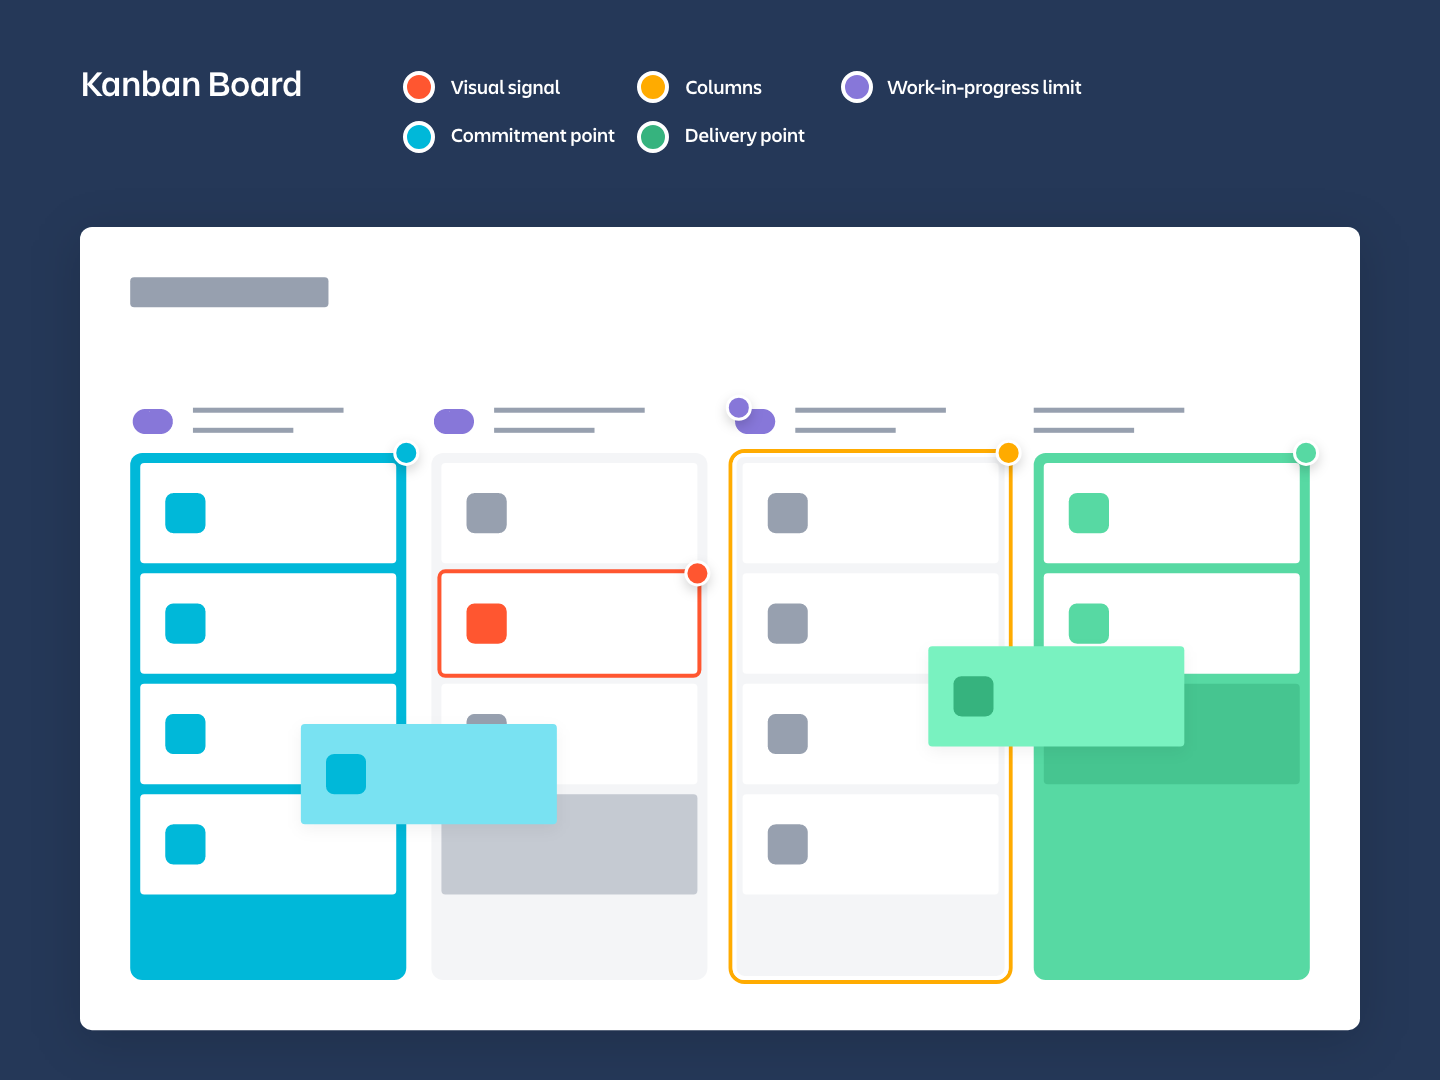
\includegraphics[scale=0.25]{img/obr4.png}
    \caption{Jednoduchá kanbasnká nástenka \cite{kaban_board}}
    \label{fig:kab-nas}
\end{figure}

\subsubsection{História}
\indent Trello bolo spustené v roku 2011 spoločnosťou Fog Creek. Za celou myšlienkou bol hlavne zakladateľ spoločnosti Joel Spolsky. Magazín Wired zaradil aplikáciu do „The 7 Coolest Startups You Haven´t Heard of Yet“ – Najlepších 7 startupov, o ktorých ste nepočuli. Tak isto sa v článku objavil názor, že Trello uľahčuje a svojim spôsobom spríjemňuje prácu na projektoch. 

\indent V máji 2016 ohlásilo Trello, že dosiahlo 1,1 milióna aktívnych používateľov denne a 14 miliónov celkovo založených účtov. V januári 2017 spoločnosť Atlassian kúpila Trello za 425 miliónov dolárov s tým, že 22\% podielu stále ostávala v rukách investorov a zakladateľa Joela Spolskeho. V roku 2019 nastal rapídny nárast používateľov, kedy ešte v marci malo Trello 35 miliónov používateľov, ale už v októbri to bolo 50 miliónov \cite{trello}.
\subsubsection{Používateľské rozhranie}
\indent Prostredie aplikácie je veľmi jednoduché na používanie a nemá v sebe veľa zbytočných vecí. Tak isto navigácia v prostredí je veľmi jednoduchá a intuitívna. Registrácia je veľmi jednoduchá. Jediné čo nový používateľ potrebuje je meno, heslo a email. 

\indent Hneď po prihlásení sa používateľovi zobrazí nástenka, kde vidí tímy, v ktorých je pridaný. Tak isto môže vytvoriť novú kartu tímu. Po vytvorení sa otvorí okno tímu, ktoré zväčša pozostáva z 3 stĺpcov – To Do, Doing a Done, plus možnosť pridať ďalšie stĺpce. Tri dopredu vytvorené stĺpce sa samozrejme dajú vymazať alebo premenovať. 

\begin{figure}[H]
    \centering
    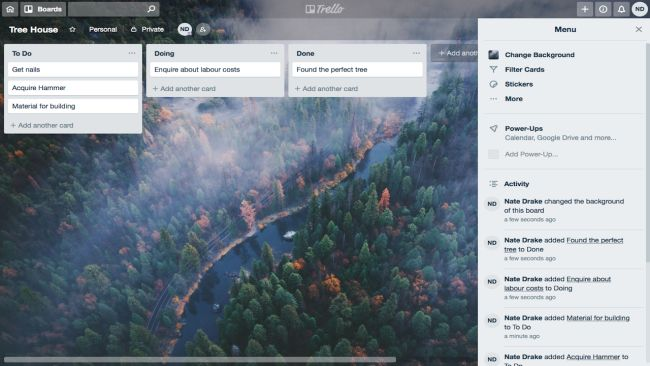
\includegraphics[scale=0.65]{img/obr-trello.jpg}
    \caption{Náhľad nástenky v aplikácii Trello \cite{trello}}
    \label{fig:nastenka}
\end{figure}

\indent V jednotlivých stĺpcoch je potom možné vytvárať nové karty, ktoré reprezentujú nejakú úlohu, komunikáciu alebo čokoľvek čo tím potrebuje. Po kliknutí na kartu sa zobrazí okno kde sa nachádza popis karty, komentáre a možnosti čo sa dá s kartou robiť – priradiť kartu používateľom aby pri zmene na karte dostali upozornenie. Upozornenia sa dajú samozrejme aj vypnúť. Na jednotlivé nástenky je možné pridanie rôznych doplnkov ako je napríklad kalendár, Google drive, Slack, Mapy alebo špecifické doplnky. 

\indent Po kliknutí na profil sa otvorí stránka používateľského profilu. Tu je možne zmeniť meno, pridať fotku profilu, zmeniť iniciály, zmeniť avatara z iniciálok na fotku, nastaviť politiku upozornení alebo pre farboslepých používateľov je možnosť zapnutia módu pre nich \cite{trello_use}. 

\begin{figure}[H]
    \centering
    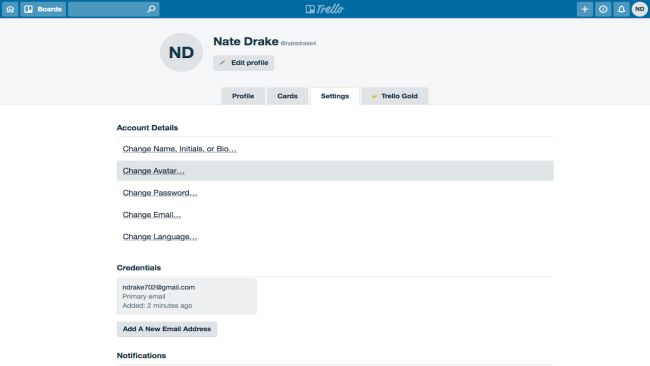
\includegraphics[scale=0.65]{img/obr-trello-profil.jpg}
    \caption{Stránka profilu v aplikácii Trello \cite{trello}}
    \label{fig:profil}
\end{figure}

\subsubsection{Doplnky}
\indent Do jednotlivých násteniek alebo tímov sa dajú pridať rôzne doplnky, ktoré rozširujú možnosti použitia Trella. Okrem rôznych Botov, ktorí len posielajú preddefinované správy alebo upozornenia, je ponuka doplnkov veľmi veľká – od štandardných doplnkov ako je kalendár, Dropbox, Google Drive, Slack, GitHub, až po špecifické, určené nie len na co-working ako napríklad Card Family, Prize Checker, Prize Tag a iné. 
\subsubsection{Cena}
\indent Trello ponúka 3 typy účtov. Bezplatný, ktorý zahŕňa neobmedzený počet násteniek, kariet, členov tímu alebo príloh. Je možné pridať jeden doplnok na nástenku a tiež pridanie prílohy o veľkosti do 10MB alebo prepojiť akýkoľvek súbor z Google Drive, Dropbox alebo OneDrive účtom. 

\indent Business balík stojí 9,99\$ mesačne, ale platí sa ročné predplatné. Balík ponúka to isté, čo bezplatný balík s tým, že je možné pridať neobmedzený počet doplnkov na nástenku a tiež pridať 250MB prílohy. Ďalšími rozširujúcimi vecami je možnosť usporiadania násteniek do kolekcií, nastaviť, kto tieto kolekcie môže vidieť alebo nahratie vlastných pozadí pre nástenky. 

\indent Enterprise balík stojí 20,83\$ mesačne, pri ročnom predplatnom. Balík zahŕňa funkcionalitu Business balíka, plus dvojfaktorová autentifikácia, šifrovanie súborov, vlastná kontrola zabezpečenia, vylepšené SLA \cite{trello}. 

\subsection{Nedostatky aplikácii}
\indent Pri každej aplikácii, okrem Facebook Workplace, sme mohli vidieť, že využívajú rôzne doplnky. Pre použitie týchto doplnkov musí používateľ zväčša disponovať účtom založeným v danej platforme doplnku. Napríklad, ak chce používateľ v Slacku využívať Google kalendár, musí mať založený účet na platforme Google. Táto skutočnosť je častokrát medzi používateľmi považovaná za otravnú a častokrát má používateľ zbytočne vytvorené účty na veľkom množstve platform, ktoré zvyknú používateľa aj spamovať na email. Preto do našej aplikácie chceme importovať služby, ktoré sú zväčša najžiadanejšie medzi službami ponúkanými ako doplnky. 

\indent Druhým veľkým nedostatkom, ktorý by sme chceli našou aplikáciou odstrániť je nutnosť platenia. Je samozrejmé, že pre veľké firmy nie je problém si radšej priplatiť za stabilnú a 100\% funkčnú aplikáciu, ktorá poskytuje veľké množstvo služieb aj za cenu pridania veľkého množstva doplnkov, ale pre študentov je odstránenie potreby platenia za aplikáciu veľkým prínosom. Jedná sa hlavne o odstránenie limitu používateľov bez poplatku za aplikáciu. Pri niektorých aplikáciách je poplatok aj za určité služby v podobe doplnkov. Toto sa v našej aplikácii tak isto nachádzať nebude. Každý používateľ bude mať plný a rovnaký prístup k aplikácii. Za základ našej aplikácie sme si zvolili rovnakú funkcionalitu ako má Slack bez doplnkov, čiže vytvorenie tímov a komunikácia v nich. K tomu pridáme funkcionalitu doplnkov, ako je kalendár s udalosťami a jednoduchú nástenku úloh v tíme, podobnú ako má Trello. 

\section{Možné technické problémy}
\indent Pri tvorbe akéhokoľvek softvéru sa vývojár stretne s množstvom situácii, ktoré môžu vyvolať pri používaní vyvýjaného softvéru problém. Preto musí vývojár už počas vyvýjania tohto softvéru tieto možné problémy odstrániť. V tejto kapitole sa preto budeme venovať možným technickým problémom, ktoré sa môžu vyskytnúť v našej pripravovanej aplikácii a načrtneme, ako tieto problémy plánujeme odstrániť.

\indent Preto, aby sme správne identifikovali možné problémy, najskôr si musíme povedať, ako bude naša aplikácia vyvýjaná. Po zvážení sme sa rozhodli, že aplikácia bude vyvýjaná princípom web-aplikácies s tým, že bude mať na pozadí aj serverovú časť, ktorá bude zodpovedná za komunikáciu s databázou.

\subsection{Používateľské rozhranie}
\indent Pred pár rokmi pri vývoji web-aplikácii sa vývojár nemusel zamýšľať nad tým, na akom zariadení bude používateľ spúšťať web-aplikáciu ( smartfóny neexistovali ) a jediné zariadenie, na ktorom mohol používateľ otvoriť web-aplikáciu, bol počitač cez prehliadač. Dnes treba myslieť na to, že používateľ môže aplikáciu otvárať na smartfóne, tablete alebo inom zariadení. Preto musia byť web-aplikácie vyvýjané spôsobom, aby sa zobrazovaná stránka vedela natívne prispôsobiť veľkosti obrazovky, na ktorej je zobrazovaná.

\indent Ďaľším faktorom je intuitívnosť využívania aplikácie. V dnešnej dobe sú v obľube jednoduché aplikácie, ktoré vie používateľ intuitívne používať. Či už sa jedná o prehľadnosť aplikácie alebo o navigáciu v aplikácii. Pokiaľ si využívanie aplikácie žiada dopodrobna si preštudovať, ako aplikáciu používať, aplikácia stratí lojalitu používateľov. 

\indent Na odstránenie toho potencionálneho problému sme sa rozhodli našu aplikáciu vyvýjať v prostredi Ionic, ktoré nám umožňuje aplikáciu vyvýjať zároveň pre viac platform. V Ionicu je možné aplikáciu vyvýjať pre štandardný webový prehliadač, zároveň je aplikácia vyvýjaná aj pre webové prehliadače v smartfónoch a tabletoch. Samozrejme, že je ale potrebné využívanie responzívných prvkov a elementov, aby sa vedeli automaticky prispôsobiť veľkosti obrazovky. Pred začatím vývoja sme sa dohodli web-aplikáciu po implementovaní vyexportovať pomocou frameworku Electron do štandarnej aplikácie pre platformu Windows. Pomocou Electronu je možné aplikáciu vyexportovať na akúkoľvek platfomu, či už Linux, MacOS, Android alebo aj iOS len zmenou príkazu na exportovanie. Týmto by sa mal tento potencionálny problém s používateľským rozhraním odstrániť.

\subsection{Používateľské skúsenosti}
\indent Používateľia sa pri prechode na novú aplikáciu obávajú hlavne o to, či ju budú vedieť používať. Preto v dnešnej dobe sa častokrát veľa aplikácii zameraných na určitú potrebu používateľa veľmi podobá. Je to hlavne preto, aby používateľ mohol hneď s aplikáciou pracovať a nemusel sa učiť, ako ju používať. Tento problém bol už čiatočne spomenutý pri probléme s používateľským rozhraním, nakoľko je to s ním úzko späté. Na odstránenie tohto problému sme sa preto rozhodli vyvýjať našu aplikáciu tak, aby bola podobná aplikácii Slack, čo sa týka vizuálnej stránky. Používateľ, ktorý používal už v minulosti aplikáciu Slack bude hneď vedieť, ako využívať aj našu aplikáciu a tak isto bude design našej aplikácie prispôsobený tak, aby aj používateľ, ktorý nevyužíval podobnú aplikáciu hneď vedel, ako našu aplikáciu využívať.

\subsection{Výkon}
\indent Rýchlosť načítavania aplikácie a celková rýchlosť jednotlivých služieb, ktoré aplikácia ponúka, je jedným z hlavných faktorov na prilákanie používateľov. Preto je potrebné aplikáciu vyvýjať tak, aby jednotlivé služby neboli náročné na či už výpočtový čas alebo na hardvér zariadenia, na ktorom aplikácia beží. 

\indent Na odstránenie tohto problému bude preto potrebné aplikáciu implemenovať bez zbytočných chýb v kóde a písať kód čo najjednoduchšie. Tak isto bude potrebné, aby sme nevyužívali príliš náročné doplnky. Pri tomto probléme bude tiež potrebné dbať na rýchlosť načítavania a ukladania do databázy. Po preštudovaní viac potencionálne využiteľných databáz sme sa rozhodli využiť databázu CouchDB s replikovaním na lokálnu databázu PouchDB. Toto využitie dvoch databáz rozoberieme pri probléme so stratou pripojenia na internet.

\subsection{Strata pripojenia na internet}
\indent Tento problém môže nastať ktorémukoľvek používateľovi. Ako sme už vyššie spomenuli, naša aplikácia bude vyexportovaná ako desktopová aplikácia, čiže ju pôjde spustiť bez pripojenia na internet, ale nastáva tu problém už pri prihlásení. Na prihlásenie bude potrebné byť pripojený na internet, nakoľko sa prihlasovacie údaje musia overiť s online databázou. Potom už bude možné stratiť pripojenie na internet, nakoľko využijeme replikáciu databázy na lokálnu databázu PouchDB. Táto databáza preberie všetky dáta pri prihláseni z online databázy a budeme ich môcť zobrazovať. Tak isto, hneď pri akomkoľvek zápise do online databázy, je táto lokálna databáza hneď aktualizovaná, ak je zariadenie opätovne pripojené na internet. Ak sa pripojenie stratí, bude zobrazovať len tie dáta, ktoré boli v databáze do straty pripojenia. 

\subsection{Bezpečnosť}
\indent Bezpečnosť dát, ktoré používateľ zadá, je samozrejmosťou každej stránky. Je prirodzené, že v tomto bode je dosť obtiažne zabrániť všetkým potencionálnym hrozbám. Tu je možné aj zvážiť, ktoré dáta sú dôležitejšie a ktoré menej. Za ochranu dát v databáze zodpovedá čiastočne už aj samotný softvér použitej databázy, ale treba zabezpečiť aj zariadenie, na ktorom databáza beží a dáta vytiahnuté z databázy, s ktorými sa pracuje.

\indent V našej aplikácii sme sa hlavne zamýšľali nad zabezpečením dát pri práci s nimi. Tu sme sa tiež rozhodovali, ktoré dáta bude treba zabezpečiť a ktoré nie. Za najdôležitejšie dáta sme zvolili prihlasovacie heslo používateľa. Ostatné dáta nie sú až také dôležité a aj s prihliadnutím na náročnosť aplikácie sme sa rozhdoli zabezpečiť len heslo. Heslo bude hneď pri registrácii na strane servera zašifrované pomocou prídavnej knižnice do node.js bcrypt a tak uložené do databázy. Po zašifrovaní už heslo nikdy nebude rozšifrovávané, čiže pri prihlasovaní sa zadané heslo pomocou funkcie knižnice bcrypt overí so zašifrovaným heslom a na základe toho bude overená správnosť zadaného hesla. 

\indent Zabezpečovanie servera nebudeme realizovať, keďže aplikácia bude testovaná len na lokálnom stroji. Ak by sa ďalej uvažovalo o distribúcii aplikácie, bude možné zabezpečenie servera, ako aj samotnej aplikácie rozšíriť.

\subsection{Zhrnutie}
\indent Tieto problémy sú asi najzásadnejšie a najväčšie, s ktorými sa stretneme pri vývoji aplikácie. Jedným menej zásadným problémom, ktorý ale ešte stojí za zmienku, je problém možnosti rozšírenia aplikácie. Niektoré aplikácie sú implementované tak, že je skoro nemožné k nim po vydaní dorobiť nejaké rozšírenie alebo dodatok. Pri implementovaní našej aplikácie na to budeme myslieť a bude implementovaná tak, aby sa k nej jednoducho dala dorobiť ďaľšia funkcionalita.

\section{Použité technológie}
\indent V nasledujúcej kapitole zhrnieme technológie, ktoré sme sa rozhodli použiť na implemetovanie našej aplikácie. Ku každej technológii popíšeme možnosti, ktoré plánujeme využiť, nakoľko rozpísať všetky možnosti je pre nás zbytočné.

\subsection{Node.js}
\indent Node.js je na svojich stránkach popísaný ako JavaScript, zameraný na udalosti pre tvorbu škálovateľných sieťových aplikácii. Na nasledovnom príklade jednoduchej aplikácie Hello World môžeme vidieť, že sa mnoho spojení dá zvládnuť súčasne - Obr.~\ref{fig:node_hello}. Po každom spojení sa spustí spätné volanie - callback, ale ak nie je potrebné vykonať žiadnu akciu, program bude spať, kým ho niekto nezavolá. 

\begin{figure}[H]
    \centering
    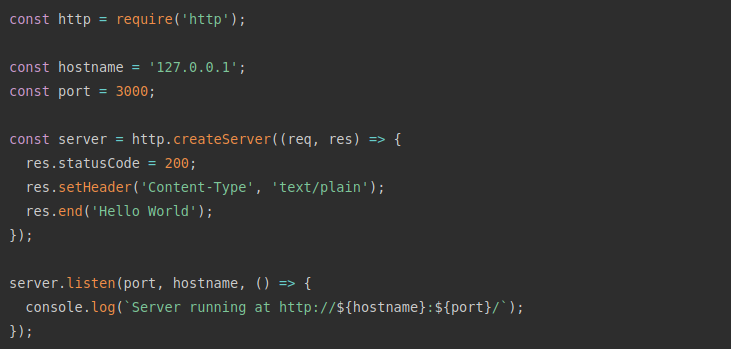
\includegraphics[scale=0.55]{img/node_hello.png}
    \caption{Jednoduchý program Hello World v Node.js \cite{nodejs_1}}
    \label{fig:node_hello}
\end{figure}

\indent Toto je v rozpore s dnešným bežnejším a modernejším prístupom založeným na vláknach operačného systému, ktoré bežia súčasne. Vytváranie vlákien pri sieťovej komunikácii je relatívne neefektívne a veľmi náročné na používanie. Mimo toho sú používatelia servera Node.js bez obáv takzvaného mŕtveho zablokovania procesu, pretože neexistujú žiadne zámky. Takmer žiadna akcia v Node.js priamo nevykonáva I/O, takže proces sa nikdy neblokuje. Preto sa odporúča na škálovateľné aplikácie používať Node.js \cite{nodejs_1}.

\subsubsection{História}
\indent Node.js bol vytvorený Ryanom Dahlom v roku 2009 a bol podporovaný len pre platformy Linux a MacOS. Pre porovanie prvé prostredie pre JavaScript na strane servera LiveWire Pro Web bolo uvedené na trh v roku 1996. Údržba a ďaľší vývoj bol najskôr vedený len samotným Dahlom, ale neskôr bol sponzorovaný firmou Joyent. Dahl prezentoval Node.js 8. Novembra 2009 na konferencii European JSConf. Node sa vtedy skladal z JavaScriptovehé enginu V8 od spoločnosti Google, udalostnej slučky (event loop) a nízko-úrovňového I/O API.

\indent V januári 2010 prišiel na trh NPM - správca balíkov pre Node.js. Tento správca umožňuje používateľom Node.js zdielanie a publikovanie zdrojových kódov doplnkových modulov. Zároveň uľahčuje ich sťahovanie, inštaláciu a aktualizáciu. Neskôr v lete 2011 Microsoft a Joyent spolupracovali na vytvorení podpory Node.js pre Windows, ktorú v tom roku aj vydali. 

\indent V roku 2014 po nezhodách pri vývoji sa časť komunity odštiepila a vytvorila io.js. O rok neskôr vznikla Node.js Foundation, ktorá zjednotila roztrieštenú komunitu a zjednotila Node.js v0.12 a io.js v3.3 do Node v4.0. Toto zjednotenie prinieslo novinky ES6 z V8 a zároveň umožnila dlhodobo trvajúci vývoj platformy.

\subsubsection{Architektúra Node.js}
\indent Každá platforma má svoju architektúru, tak isto aj Node.js. V tejto kapitole rozoberieme jej hlavné vlastnosti a časti. Nie všetky budeme potrebovať pri implementácii, ale je dobré ich poznať.

\indent Základnou vlastnosťou je, že Node.js má asynchrónne a udalostne riadené API. Toto zaručuje to, že nasledujúce volania nie sú blokované predchádzajúcim volaním. V praxi to znamená, že Node.js nikdy nečaká, kým je z volania vrátená hodnota, respektíve je volanie dokončené a ukončené. Server sa po zavolaní volania presunie na ďaľšie a vnútorný notifikačný mechanizmus udalosti dostane odpoveď z prechádzajúcich volaní vtedy, keď sú dokončené a dostane sa tým aj k výsledku. 

\indent Druhou veľkou výhodou je existencia udalostnej slučky. Vďaka tomu je jednovláknový a vysoko škálovateľný. Vyššie spomínaný udalostný mechanizmus napomáha serveru vrátiť odpoveď bez blokovania. Tým sa server stáva vysoko škálovateľný v porovnaní s tradičnými riešeniami na strane servera, ktoré majú obmedzený počet vlákien a tým sa aj počet požiadaviek, ktoré sú spracované súčasne, stáva obmedzený. 

\indent Ďaľšou výhodou je, že aplikácie založené na platforme Node.js sú bez vyrovnávacej pamäte, čiže údaje, posielané na výstup, sú zoskupované do malých blokov.

\indent Na Obr.~\ref{fig:node_arch} môžeme vidieť základné rozdelenie architektúry platformy Node.js. 

\begin{figure}[H]
    \centering
    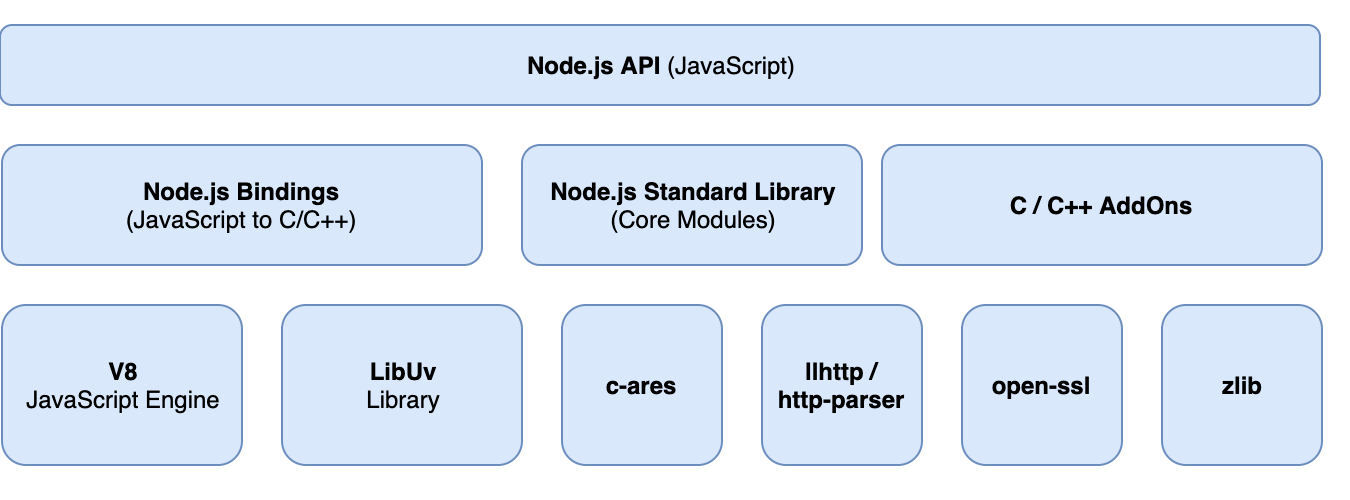
\includegraphics[scale=0.30]{img/node_architecture.png}
    \caption{Architektúra platformy Node.js \cite{nodejs_3}}
    \label{fig:node_arch}
\end{figure}

\indent Na vrchole sa nachádza Node.js API, ktoré je napísané v JavaScripte a je možné k nemu priamo pristupovať za účelom využitia v aplikáciach. Pod API sa nachádza trio Node.js Bindings, Node.js Standard Libraries a C/C++ AddOns. Node.js Standard Libraries sú funkcie súvisiace s knižnicami operačného systému a umožňujú využívanie napríklad časovačov, súborového systému alebo sieťových volaní http. Node.js Bindings je knižnica, ktorá umožňuje komunikáciu JavaScriptu s C/C++ a tým ich viaže dokopy. Poslednou časťou sú C/C++ AddOns, čo sú dynamicky linkované doplnky viazané na C/C++ knižnice. Toto umožňuje vytvorenie akejkoľvek C/C++ knižnice a jej využitie v Node.js \cite{nodejs_3,nodejs_4}. 

\indent Na spodku sa náchádzajú knižnice C/C++:
\begin{itemize}
    \item V8 JavaScript Engine - konvertuje JavaScript do strojového kódu daného operačného systému
    \item LibUv - multiplatformová C knižnica zameriavajúca sa na asynchrónne I/O operácie
    \item c-ares - C knižnica pre asynchrónne DNS požiadavky a odpovede
    \item http-parser - C knižnica pre HTTP požiadavky a odpovede
    \item open-ssl - kryptografické funkcie
    \item zlib - C knižnica pre synchrónnu aj asynchrónnu kompresiu, dekompresiu a pre streamovanie dát 
\end{itemize}

\subsubsection{Event loop}
\indent Event loop alebo udalostná slučka je to, čo umožnuje Node.js vykonávať neblokujúce vstupno-výstupné operácie napriek tomu, že JavaScript je jednovláknový. Keďže väčšina moderných jadier má viacvláknové spracovanie, tak môžu zvládnuť vykonávať viac operácii na pozadí. V Node.js to ale funguje tak, že keď je jedna z operácii dokončená, jadro povie Node.js, aby do fronty na vykonanie pridalo príslušné spätné volanie na výsledok vykonanej operácie. Na Obr.~\ref{fig:event_loop} môžeme vidieť zjednodušený diagram, ako to funguje. 

\begin{figure}[H]
    \centering
    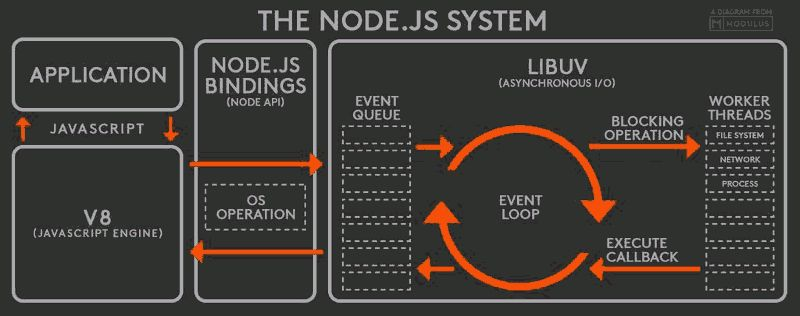
\includegraphics[scale=0.55]{img/evet_loop.jpg}
    \caption{Zjednodušená verzia fungovania Node.js architektúry \cite{nodejs_2}}
    \label{fig:event_loop}
\end{figure}

\indent Keď sa Node.js spustí tak inicializuje slučku udalostí a spustí poskytnutý vstupný skript, ktorý môže uskutočňovať asynchrónne volania API. Následne sa začne spracovávať slučka udalostí. Tá postupne spracováva udalosti z fronty udalostí bez toho, aby čakala na dokončenie daných udalostí. Keď je táto udalosť hotová, tak sa jej spätné volanie zaradí na spodok fronty udalostí a jej výsledok je teda znova spracovaný, keď sa k nemu slučka dostane. Toto sa opakuje kým nie je fronta udalostí vyčerpaná alebo nie je dosiahnutý maximálny počet spätných volaní \cite{nodejs_2}. 

\subsubsection{Nevýhody Node.js}
\indent Ako sme vyššie popísali, Node.js má veľké množstvo výhod, medzi ktoré hlavne patrí asynchrónne I/O, škalovateľnosť, veľká a aktívna komunita a veľké množstvo prídavných modulou. Avšak Node.js má aj určité nevýhody. Medzi hlavné patrí:
\begin{itemize}
    \item neefektívnosť pri náročných procesoch pre CPU - tvorba reportov, analýz, zložité výpočty... 
    \item nepochopenie práce s callbackmi môže viesť používanie Node.js k zle napísaným kódom
    \item menej štandarných knižníc v porovnaní s klasickou Javou a .NET platformou
\end{itemize}

\indent Môžeme teda vidieť, že nie vždy je využitie Node.js možnosťou. Veľmi záleží akú aplikáciu vyvíjame. Ak pracujeme na aplikácii pre real-time komunikáciu s využitím websocketov, streaming alebo rýchlu prácu so súbormi, tak je Node.js veľmi vhodný. 

\subsection{Node Package Manager}
\indent Node package manager, skrátene len NPM, je správca prídavných balíkov vyvinutý pre Node.js. Oficiálna stránka \textit{https://www.npmjs.com} obsahuje tisícky voľných balíkov na stiahnutie a používanie. NPM program sa automaticky naištaluje pri inštalácii Node.js. NPM sa následne dá spúšťať z príkazového riadku. Tak isto je možné vytvorenie vlastného balíka a nahratie ho do centrálneho repozitára oficiálnej stránky NPM.

\indent Balík v Node.js je zväčša adresár obsahujúci všetky súbory, ktoré pridavný modul potrebuje. Modul je JavaScriptová knižnica, ktorú programátor môže pridať do svojho projektu. Jedným zo súborov, ktoré sa nachádzajú v adresári, musí byť metadátový súbor s názvom \textit{package.json}. V tomto súbore sú definové vlastnosti, meno a verzia balíka. Na Obr.~\ref{fig:package} môžeme vidieť, ako takýto súbor vyzerá \cite{npm,npm_node}.  

\begin{figure}[H]
    \centering
    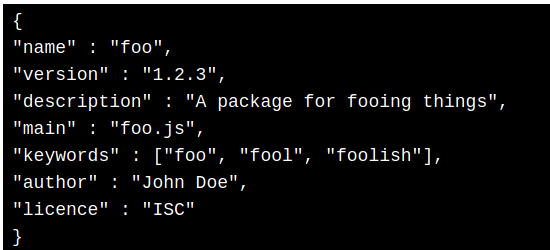
\includegraphics[scale=0.55]{img/package.png}
    \caption{Jednoduchý \textit{package.json} súbor \cite{npm}}
    \label{fig:package}
\end{figure}

Inštalácia balíkov sa dá zrealizovať tromi spôsobmi:
\begin{itemize}
    \item manuálna inštalácia len pre projekt, na ktorom pracujeme - v termináli sa v priečinku projektu zavolá príkaz \textbf{npm instal \textit{názov\char`_modulu}}. Posledná verzia balíka sa nainštaluje pre projekt a uloží do adresára \textit{node\char`_modules}.
    \item manuálna inštalácia globálne pre systém - v termináli sa zavolá príkaz \textbf{npm instal \textit{názov\char`_modulu} -g}. Táto možnosť sa ale neodporúča.
    \item poslednou možnosťou je dopísanie do projektového suború \textit{package.json} do časti dependencies názov modulu a jeho verziu a v termináli zadať príkaz \textbf{npm install}.
\end{itemize}

\subsection{Ionic framework}
\indent Ionic je voľne dostupné, open-source prostredie na vytváranie hybridných aplikácii pre mobilné zariadenia vytvorené Maxom Lynchom a Adamom Bradleym zo spoločnosti Drifty Co. v roku 2013. Prvá verzia vydaná z roku 2013 bola založená na AngularJS a Apache Cordova, avšak najnovšia verzia bola prepracovaná ako skupina webových komponentov, čo umožňuje programátorom zvoliť pri tvorbe aplikácie ľubovolný framework ako je napríklad Angular, React alebo Vue.js. Je ale tiež možné zvoliť natívne Ionic componenty bez použitia akéhokoľvek iného frameworku. Ionic poskytuje nástroje a služby na tvorbu nie len mobilných aplikácii, ale aj klasických aplikácii pre Windows, MacOS alebo progresívných webových aplikácii založených na moderných spôsoboch tvorby webových aplikácii pomocou CSS, HTML a Sass.

\subsubsection{Služby a vlastnosti}
\indent Ionic používa doplnok Cordovu alebo novší Capacitor na získanie prístupu k operačnému systému zariadenia, na ktorom aplikácia beží a tým aplikácia vie pristupovať k perifériám zariadenia, ako je napríklad GPS modul, kamera alebo baterka. Tieto perifériá potom môže aplikácia využívať pre svoju funkčnosť. \newline
\textbf{Capacitor}\newline
\indent Capacitor je open-source projekt, ktorý umožňuje spúšťanie moderných web aplikácii natívne na operačných systémoch Android alebo iOS, prípadne s využitím Electronu na systémoch Windows, MacOS. Tiež poskytuje výkonné a ľahko použiteľné rozhranie pre prístup k natívnym SDK a API na každej platforme. O Capacitore sa hovorí ako o výkonnom novom prehliadači webových aplikácii, ktorý odomkne celú natívnu funkčnosť každej platfromy prostredníctvom konzistentných API medzi platformami. S použitím Capacitora nemusí vývojár spravovať viac rozhraní API pre každú platformu, ale môže namiesto toho vyvíjať aplikáciu ako celok, bez nutnosti uvažovať na akej platforme bude aplikácia spustená \cite{ionic}. \newline
\textbf{Cordova}\newline
\indent Podobne ako Capacitor je Cordova open-source projekt umožňujúci spustenie web apliikácie na rôznych platformách. Narozdiel od Capacitoru nie je Cordova prispôsobená na využitie Electronu pre export na desktopovú aplikáciu. Preto sa dnes už viacej využíva novší Capacitor \cite{ionic}.

\indent Ionic využíva všetky doteraz dostupné webové komponenty s tým, že ich funkčnosť zrýchľuje a robí ju menej náročnú pre zariadenie, na ktorom aplikácia beží. Tak isto, ako bolo už vyššie spomenuté, umožňuje využitie ktorýchkoľvek moderných frameworkov a ich komponentov. Pre vývojárov je k dispozícii vlastné prostredie na tvorbu Ionic aplikácii Ionic studio (Obr.~\ref{fig:ionic_studio}) a taktiež je dostupné CLI pre prácu s projektami cez príkazový riadok. 

\begin{figure}[H]
    \centering
    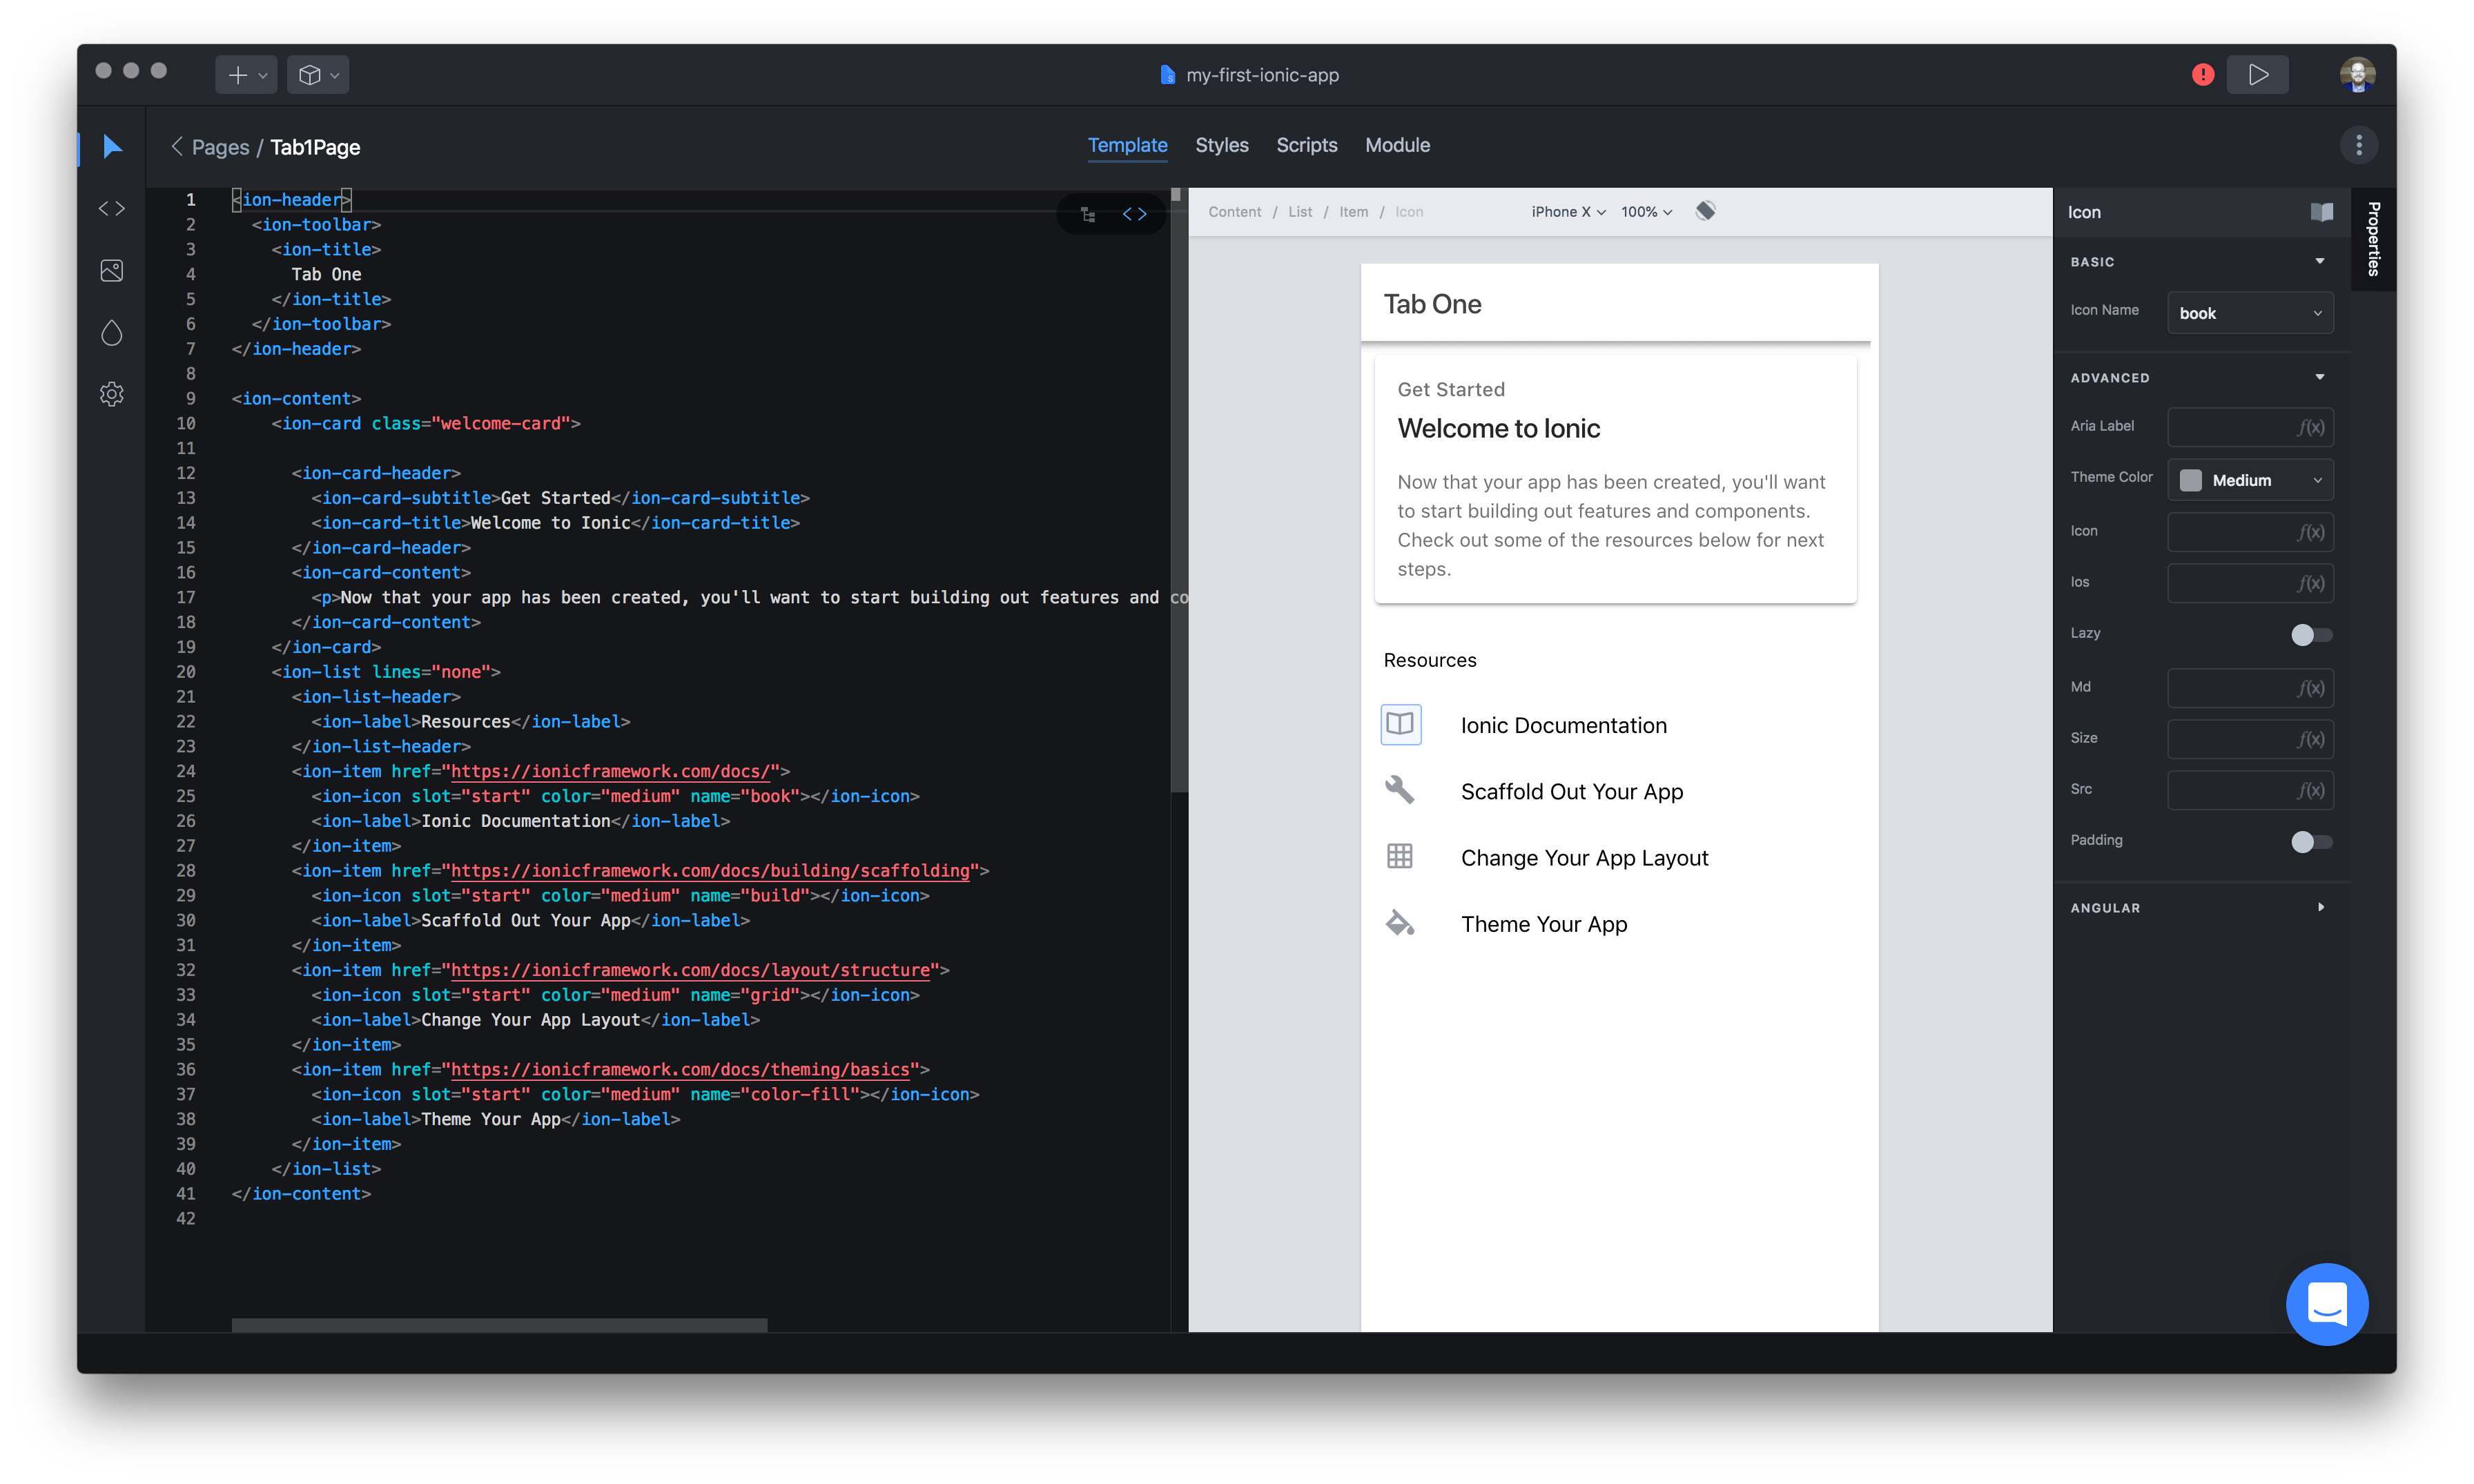
\includegraphics[scale=0.12]{img/ionic_studio.png}
    \caption{Vývojové prostredie Ionic studio}
    \label{fig:ionic_studio}
\end{figure}

\subsubsection{Inštalácia}
\indent Pri inštalácii Ionic frameworku je potrebné si povedať, že Ionic je NPM modul, čo znamená, že na jeho inštaláciu je potrebné mať nainštalovaný Node.js. Tak isto je potrebné povedať, že pomocou Ionicu je možné vyvíjať aplikácie pre mobilné operačné systémy Android verzia 4.1+ a iOS 7+, pričom treba ešte spomenúť, že pri veľkom množstve existujúcich Android zariadení je možné, že na niektorých zariadeniach vyvíjaná aplikácia nemusí dobre fungovať. Vyvíjanie aplikácii pomocou Ionicu je možné na ktoromoľvek operačnom systéme - Windows, Linux, MacOS. 

\indent Prvým krokom pri inštalácii je nainšalovanie Apache Cordova alebo Capacitor, ak nerátame inštaláciu Node.js. Cordova aj Capacitor sú podobne ako Ionic NPM moduly, takže ich inštalácia je jednoduchá. Po nainštalovaní Cordova respektíve Capacitor sa môže nainštalovať samotný NPM modul Ionic. Následne je už možné vytvoriť projekt a začať pracovať na aplikácii. Pri vytváraní projektu je ale ešte možné špecifikovať framework, aký chceme na vývoj aplikácie použiť. Toto sa realizuje príkazom \textit{ionic start nazov\char`_aplikacie --type=angular --capacitor}. Tu si všimnime, že do prepínača type sa zadal angular, čiže aplikácia bude vyvíjaná pomocou frameworku Angular a bude sa používať Capacitor. Keďže Ionic je NPM modul, je samozrejmé, že do aplikácie je možné doinštalovať takmer akýkoľvek ďaľší NPM modul na rozšírenie funkčnosti aplikácie. Pri vývoji aplikácie je ešte potrebné pomocou doplnku Cordova alebo Capacitor špecifikovať na akej platforme má aplikácia fungovať. Toto sa urobí príkazom \textit{ionic cordova/capacitor platform add ios/android} zadaným do príkazového riadku. Je možné pridať aj obidve platfromy. 

\subsection{Angular}
\indent Angular je framework na vyvíjanie webových aplikácii vyvinutý a spravovaný spoločnosťou Google. Googlom je označovaný ako \textit{"Super framework založený na JavaScripte pre čokoľvek"}. Takto bola označovaná jeho prvá verzia AngularJS, ktorá bola založená na JavaScripte. Dnes je však používanejšia jeho druhá verzia Angular 2+, označovaná tiež ako Angular, čo označuje všetky verzie od verzie 2, ktoré sú narozdiel od prvej verzie založené už na TypeScripte. Hneď po svojom vydaní sa Angular stal jedným z najviac používaných frameworkov pre tvorbu web aplikácii na trhu. Tento úspech je založený hlavne na tom, že narozdiel iných frameworkov doby, keď Angular vyšiel, je Angular výlučne objektovo-orientovaný a jeho syntax je prekvapivo blízky Jave 8, aj keď je založený na TypeScripte \cite{bakalarska_praca,angular_1,angular_2}. 

\subsubsection{História}
\indent Prvá verzia AngularJS bola vydaná ešte v roku 2010. Ako bolo vyšie spomenuté, táto verzia bola založená na JavaScripte. Aj keď po vydaní novšej verzie Angular 2 väčšina vývojárov prešla na novšiu verziu, AngularJS je stále udržiavaný framework so stálou podporou nových aktualizácii a živou komunitou vývojárov. 

\indent Na konci roka 2014 Google ohlásil, že pracuje na novej verzii frameworku Angular 2, ktorý bude kompletne prepísaný AngularJS do novo vyvýjaného jazyka ArtScript. Po ohlásení však Microsoft súhlasil s pridaním podpory pre nimi vyvíjaný TypeScript a tak bol Angular 2 založený ako TypeScriptový framework. Zaujímavosťou je, že hneď od vydania Angularu 2 bolo možné v ňom vývíjať aplikácie aj v JavaScripte, nakoľko má Angular 2 podporu aj JavaScriptu. Oficiálne bol Angular 2 vydaný 14. septembra 2016, aj keď ako beta verzia fungoval už od roku 2015. 

\indent Na konci roka 2016 bol ohlásený Angular 4 ako nástupca Angularu 2. Označenie 3 bolo preskočené, aby sa zabránilo nezrovnalostiam z dôvodu, že nové aktualizácie Angularu 2 boli označované ako v3.3.0. Angular 4 bol oficálne vydaný 23. marca 2017 a priniesol novinky ako HttpClient - vylepšená knižnica pre vytváranie HTTP požiadaviek, nový životný cyklus udalostí a iné menšie vylepšenia. 

\indent Dnes je už vydaná verzia 9, pričom každá verzia (5,6,7,8) priniesla vždy hlavne podporu nových Material Dizajnov, podporu nových knižníc a podporu tvorby progresívnych web aplikácii. Google sa pri vydávaní nových aktualizácii zaručil, že každá nová verzia bude spätne kompatibilná a nové verzie chce vydávať dva krát ročne \cite{bakalarska_praca,angular_1}.

\subsubsection{Architektúra}
\indent Základ Angularu tvoria NgModuly. Tieto moduly poskytujú kompiláciu komponentov, čo sú druhá základná zložka architektúry Angularu. NgModuly zhlukujú súvisiace kódy do množín, ktoré majú spoločnú funkcionalitu. Skrátene sa dá povedať, že každá aplikácia je definovaná množinou NgModulov. Základom každej aplikácie je jeden koreňový NgModul, ktorý môže mať pod sebou ľubovolný počet ďaľších NgModulov. Tento koreňový modul umožňuje navigáciu v aplikácii a bootstraping. 

\indent Ako bolo vyššie spomenuté, druhým stavebným prvkom sú komponenty. Komponenty zodpovedajú za to, čo sa zobrazuje na obrazovke používateľa. Rovnako, ako pri NgModuloch, aj komponenty musia mať jeden koreňový komponent, ktorý potom v sebe má usporiadané ďalšie komponenty. Komponenty v sebe používajú aj služby, ktoré poskytujú špecifické funkcie, ktoré nie vždy priamo súvisia so zobrazením. Poskytovatelia týchto služieb sú vkladaní do komponentov ako závislosti. Týmto sa stáva kód modulárnym, opakovateľne použiteľným a efektívnym. Komponenty aj služby do nich vkladané sú označované dekorátormi, ktoré určujú, o aký typ komponentu a služby ide a poskytujú taktiež metadáta, ktoré hovoria o tom, ako tieto komponenty a služby používať. Metadáta tiež spájajú komponenty so šablónami, ktoré definujú, ako budú komponenty zobrazené na jednotlivých stránkach. Šablóna je kombinácia obyčajných kódov HTML so smernicami Angularu, čo umožňuje Angularu úpravu tohto HTML kódu ešte pred jeho zobrazením v okne prehliadača \cite{angular_3}. 

\begin{figure}[H]
    \centering
    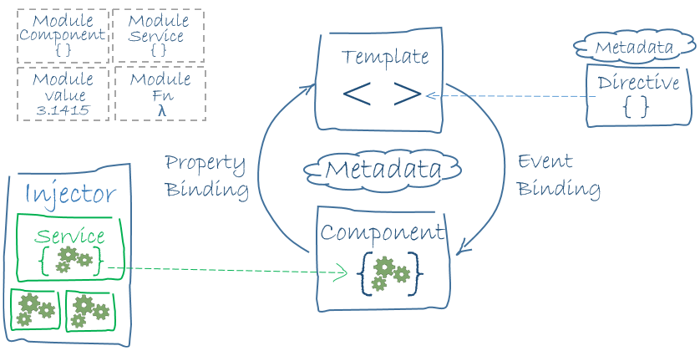
\includegraphics[scale=0.5]{img/angular_architecture.png}
    \caption{Princíp fungovania Angularu \cite{angular_3}}
    \label{fig:angular_architecture}
\end{figure}

\newpage

\subsubsection{Výhody Angularu}
\noindent\textbf{Komponentová architektúra, ktorá poskytuje vyššiu kvalitu kódu}

\indent  Architektúra založená na komponentoch je jednou z vecí, ktorá robí rozdiel medzi AngularJS a jeho nástupcom. Angular komponenty možno považovať za malé časti používateľského rozhrania alebo ako časť aplikácie. Aj keď je každý komponent zapuzdrený so svojou funkčnosťou, v Angulare existuje prísna hierarchia komponentov. Napríklad v Angular 9 boli predstavené komponenty Mapy Google a YouTube Player.

\indent Zatiaľ čo AngularJS bol postavený hlavne na architektúre Model-View-Controller (MVC), počnúc verziou 2 sa Angular považuje za komponentovo-založený, čo je veľmi podobné MVC, ale zaisťuje to vyššiu opätovnú použiteľnosť komponentov v celej aplikácii. To umožňuje vytváranie používateľských rozhraní s mnohými pohyblivými časťami a zároveň zrýchľuje priebeh vývoja aplikácie \cite{angular_1}. \newline
\textbf{TypeScript: lepšie nástroje, čistejší kód a vyššia škálovateľnosť}

\indent Angular je písaný pomocou TypeScript jazyka, ktorý je v podstate nadradený JavaScriptu. Plne sa skompiluje do JavaScriptu, ale pomáha pri zisťovaní a odstraňovaní bežných chýb pri písaní kódu. Aj keď malé projekty JavaScriptu takéto vylepšenie nevyžadujú, podnikové aplikácie vyzývajú vývojárov, aby vylepšili svoj kód a častejšie overovali jeho kvalitu.

\indent V Angulari píšeme komponenty v TypeScript, šablóny v HTML a rozširujeme ich pomocou Angularu. Takto funguje väčšina JS frameworkov. Šablóny HTML sa potom skompilujú do pokynov jazyka JavaScript, takže TypeScript alebo JS sú naše hlavné nástroje na prácu v Angulari. Victor Savkin, bývalý vývojár tímu Google Angular, vysvetľuje, že prechod z jazyka JavaScript do jazyka TypeScript je opodstatnený nástrojmi pre veľké projekty v podnikovom meradle. TypeScript má lepšie služby navigácie, automatického dopĺňania a refaktoring \cite{angular_1}.\newline
\textbf{RxJS: efektívne asynchrónne programovanie}

\indent RxJS je knižnica bežne používaná v Angular na spracovanie asynchrónnych dátových volaní. Umožňuje nezávisle a paralelne spracovávať udalosti a čakať na vykonanie nejakej udalosti a ponechať webovú stránku nereagujúcu. V zásade to funguje ako montážna linka, kde sa vykonávanie rozdeľuje na jednotlivé a vymeniteľné kusy a nie je viazaná na jednu osobu. Je samozrejmé, že už pred RxJS existovalo asynchrónne programovanie, ale táto knižnica uľahčila veľa vecí \cite{angular_1}.\newline
\textbf{Dlhodobá podpora}

\indent Niektorí softvéroví inžinieri považujú samotnú skutočnosť, že spoločnosť Google podporuje technológiu Angular, za hlavnú výhodu tejto technológie. Dobrým znamením je, že spoločnosť Google oznámila dlhodobú podporu pre túto technológiu. Inžinieri Igor Minar a Steven Fluin, stojaci za Angularom, potvrdili tento záväzok v hlavnom vystúpení NG-Conf 2017. V zásade to znamená, že spoločnosť Google plánuje držať sa Angularu a ďalej ho rozvíjať a snažiť sa udržať vedúce postavenie medzi front-end inžinierskymi nástrojmi \cite{angular_1}.\newline
\textbf{Silná komunita}

\indent Keďže je tu Angular už zopár rokov je jasné, že za ten čas vznikla veľká a živá komunita, ktorá denodenne prináša nové balíky, vylepšenia, návody, rady a iné užitočné veci pri práci s Angularom. Ak sa priemerný inžinier stratí alebo má problém pri vývoji aplikácie, vždy existuje nástroj, ktorý pomôže vyriešiť problém, ktorý sa objaví \cite{angular_1}.

\subsection{Electron}
\indent Electron je populárny framework, ktorý umožnňuje vytváranie desktopových aplikácií pre MacOS, Linux alebo Windows pomocou známych webových technológií HTML, JavaScript a CSS vytvorený a udržiavaný firmou GitHub. Niektoré veľmi populárne desktopové aplikácie, ako sú Visual Studio Code a Slack, sú vytvorené pomocou frameworku Electron. Electron je založený na prehliadači Chromium pre interpretáciu používateľského rozhrania na Node.js pre prístup k súborovým systémom. Pretože spoločnosť Electron nám poskytuje webové rozhranie pre webové aplikácie, môžeme na vývoj aplikácií pre osobné počítače použiť akýkoľvek druh JavaScriptu prípadne TypeScriptu \cite{electron}.

\begin{figure}[H]
    \centering
    
\includegraphics[scale=0.35]{img/electron_aps.png}
    \caption{Firmy využívajúce vo svojich aplikáciách Electron \cite{electron}}
    \label{fig:electron_aps}
\end{figure}

\subsubsection{Architekúra}
\indent Elektronové aplikácie sa skladajú z viacerých procesov. Existuje proces „prehliadača“ a niekoľko procesov „vykreslenia“. Proces prehliadača spúšťa aplikačnú logiku a potom môže spustiť viacero procesov vykresľovania, ktoré vykresľujú okná, ktoré sa zobrazujú na obrazovke používateľa použitím HTML a CSS. Procesy prehliadača aj vykreslenia sa môžu spustiť s integráciou Node.js, ak je povolená.
\indent Väčšina rozhraní Electron API je napísaná v C ++ alebo Objective-C a potom je exponovaná priamo aplikačnému kódu prostredníctvom väzieb JS. Prvotné verzie Electronu boli náchylné na webové útoky pomocou cross-site skriptingu nakoľko je Electron založený na engine Chromium, ktorý je náchylný na tento typ útoku. Avšak neskoršími aktualizáciami frameworku Electron bola táto zraniteľnosť odstránená a vývojár sa ňou nemusí osobitne zaoberať \cite{electron}. 


\subsection{Apache CouchDB}
\indent CouchDB vyvíjaná a udržiavaná firmou Apache je open-source NoSQL databáza, ktorá zhromažďuje a ukladá údaje do dokumetov vo formáte JSON. Na rodziel od relačných databáz používa CouchDB dátový model bez schém. Tento princíp zjednodušuje správu záznamov v rôznych zariadeniach, mobilných telefónoch a webových prehliadačoch.

\indent CouchDB bola predstavená v roku 2005 a neskôr sa stala projektom firmy Apache Software Foundation v roku 2008. Ako open-source projekt je CouchDB podporovaná veľkou aktívnou komunitou vývojárov, ktorí neustále vylepšujú softvér so zameraním na jednoduché používanie webu \cite{coucdb}.

\begin{figure}[H]
    \centering
    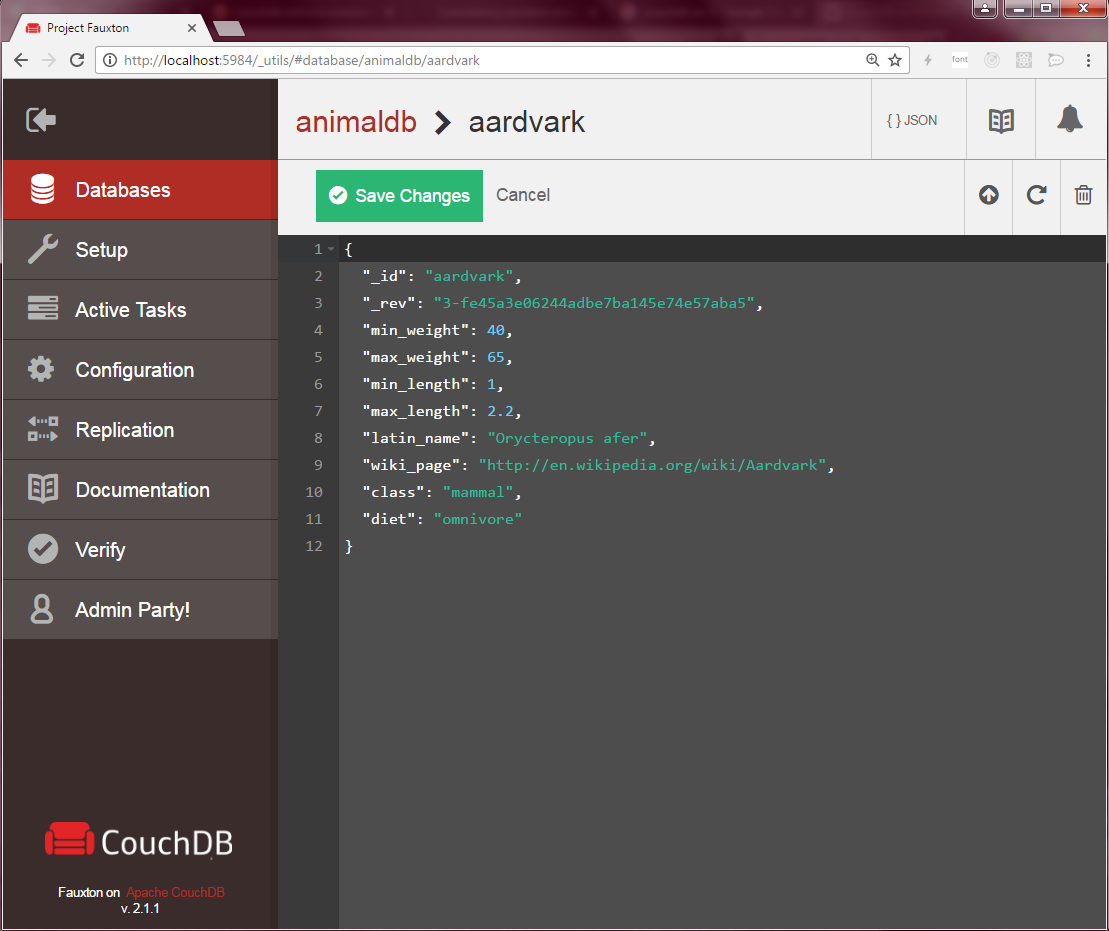
\includegraphics[scale=0.25]{img/coucdb.png}
    \caption{JSON dokument v aplikácii na správu CouchDB \cite{coucdb}}
    \label{fig:couch_db}
\end{figure}

\subsubsection{Výhody použitia CouchDB}
\indent CouchDB predstavuje celý rad výhod zameraných na používateľov a vývojárov. Motiváciu vývoja CouchDB možno definovať jedným slovom: relax. CouchDB prichádza s množstvom výhod navrhnutých na zníženie námahy pri prevádzkovaní pružného distribuovaného systému. Tu sú niektoré kľúčové vlastnosti CouchDB a ako sa líši od iných databáz NoSQL.\newline
\textbf{Škálovateľnosť} \newline
\indent Architektonický návrh CouchDB ju robí mimoriadne prispôsobivou pri rozdeľovaní databáz a meraní údajov na viacerých uzloch. CouchDB podporuje horizontálne rozdelenie a replikáciu na vytvorenie ľahko spravovaného riešenia na vyrovnanie času potrebného na načítanie aj zápis počas zavádzania databázy.

\indent CouchDB je vybavená veľmi odolným a spoľahlivým úložným enginom, ktorý bol vybudovaný od základov pre viackanálové databázové infraštruktúry. Ako NoSQL databáza je CouchDB veľmi prispôsobiteľná a otvára dvere vývoju predvídateľných aplikácií založených na výkone bez ohľadu na objem údajov alebo počet používateľov \cite{coucdb}.\newline
\textbf{Žiadne read-locks} \newline
\indent Vo väčšine relačných databáz - kde sú údaje uložené v tabuľkách - ak sa niekedy potrebuje aktualizovať alebo upraviť tabuľka, tak sa riadok zmenených údajov uzamkne pre ostatných používateľov, až kým sa nespracuje požiadavka na úpravu. Môže to spôsobiť problémy s prístupnosťou pre klientov a celkové prekážky v procesoch správy údajov.

\indent CouchDB používa MVCC na simultánnu správu prístupu k databázam. To znamená, že bez ohľadu na aktuálne načítanie databázy môže CouchDB bežať na plnú rýchlosť a bez obmedzenia pre svojich používateľov. Pretože dokumenty v CouchDB sú verziované a pripojené v reálnom čase. V požiadavkách na čítanie databázy sa vždy zobrazia najnovšie aktualizované databázové snímky, bez ohľadu na to, kto k dokumentu pristupoval ako prvý \cite{coucdb}.\newline
\textbf{CouchDB replikácia} \newline
\indent Jednou z definujúcich funkcií CouchDB je obojsmerná replikácia, ktorá umožňuje synchronizáciu údajov na viacerých serveroch a zariadeniach prostredníctvom obojsmernej replikácie. Táto replikácia umožňuje podnikom maximalizovať dostupnosť systémov, skrátiť dobu obnovy dát, lokalizovať údaje najbližšie ku koncovým používateľom a zjednodušiť procesy zálohovania.

\indent V CouchDB sa nerozlišuje, či sú dáta uložené na jednom serveri alebo na viacerých serveroch. CouchDB skôr identifikuje zmeny dokumentov, ku ktorým dôjde z akéhokoľvek zdroja, a zabezpečí, aby všetky kópie databázy zostali synchronizované s najaktuálnejšími informáciami. To umožňuje samostatnú správu a správu viacerých replík databázy a zároveň poskytuje presné informácie v reálnom čase vo viacerých počítačových prostrediach \cite{coucdb}.\newpage
\noindent\textbf{HTTP API} \newline
\indent CouchDB používa RESTful API na prístup do databázy odkiaľkoľvek, s plnou flexibilitou operácií CRUD (vytváranie, čítanie, aktualizácia, mazanie). Tento jednoduchý a efektívny spôsob pripojenia k databáze robí CouchDB flexibilnou, rýchlou a výkonnou na použitie pri zachovaní vysokej dostupnosti \cite{coucdb}.\newline
\textbf{Stavaná pre offline používanie} \newline
\indent Keď škálujeme použiteľnosť a prístupnosť databázy, je nevyhnutné vytvárať aplikácie, ktoré fungujú rovnako offline, ako online. CouchDB umožňuje aplikáciám ukladať zozbierané údaje lokálne na mobilných zariadeniach a prehliadačoch a potom ich synchronizovať, keď sa vrátia online \cite{coucdb}.

\subsection{PouchDB}
\indent PouchDB je open-source databáza JavaScript inšpirovaná Apache CouchDB, ktorá je navrhnutá tak, aby fungovala dobre v prehliadači. PouchDB bola vytvorená s cieľom pomôcť vývojárom webu vytvárať aplikácie, ktoré fungujú rovnako offline, ako online. Aplikáciám umožňuje ukladať údaje lokálne v režime offline, potom ich synchronizovať so servermi CouchDB alebo inými kompatibilnými servermi, keď je aplikácia späť online.

\indent Architektúra PouchDB je rovnaká ako pri CouchDB. Dáta sú ukladané formátom JSON a celá práca s nimi je rovnaká ako pri CouchDB. Preto sa pri online-offline aplikáciách odporúča pri použití CouchDB používať aj PouchDB \cite{poucdb}.

\begin{figure}[H]
    \centering
    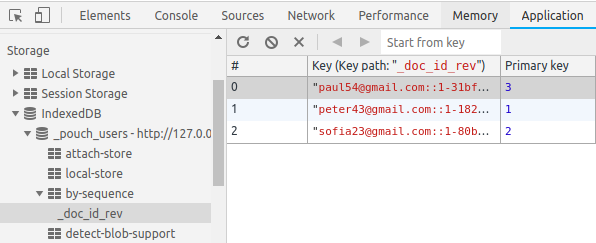
\includegraphics[scale=0.80]{img/pouchdb.png}
    \caption{Náhľad PouchDB v prehliadači Google Chrome \cite{poucdb}}
    \label{fig:pouch_db}
\end{figure}

\section{Návrh aplikácie}
\indent Témou diplomovej práce je implementovať co-working aplikáciu s využitím webového frameworku Ionic/Angular s neskorším exportom na desktopovú aplikáciu pomocou Electronu na strane frontendu a s použitím Node.js a CouchDB na strane servera. V tejto kapitole sa budeme zaoberať návrhom celej aplikácie s využitím daných technológii na jednotlivých komponentoch. 

\begin{figure}[H]
    \centering
    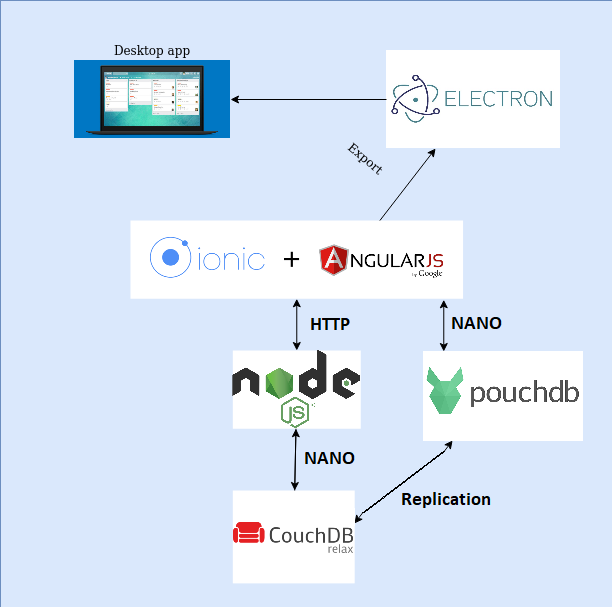
\includegraphics[scale=0.60]{img/diagram.png}
    \caption{Návrh komunikácie medzi komponentami}
    \label{fig:diagram}
\end{figure}

\indent Po prieskume aktuálnych technológii sme sa rozhodli využiť Node.js ako náš server, ktorý bude komunikovať s našou NoSql databázou CouchDB, do ktorej bude ukladať zadané dáta a zároveň posielať žiadané dáta na frontend implementovaný pomocou typescriptovo založeného frameworku Ionic. Ionic sa, ako bolo spomenuté v kapitole 4.3, využíva na tvorbu webových alebo mobilných aplikácii. Preto finálnu webovú aplikáciu exportujeme nakoniec pomocou Electronu na desktopovú aplikáciu pre platformu Windows/Linux/MacOS.

\subsection{Špecifikácia požiadaviek}
\indent Prvým krokom pri tvorbe návrhu je špecifikovanie vlastností a celkového správania aplikácie. Definuje sa tu funkcionalita, ktorú chceme aby naša aplikácia mala, správanie aplikácie v určitých situáciách a jej kľúčové parametre, ktoré musí podľa požiadaviek spĺňať.
\subsubsection{Používateľské požiadavky} 
\indent Používateľské požiadavky sa stanovili na základe prehľadu co-working aplikácii, ktoré už existujú. Za základ sa zobrali hlavné funkcionality Slacku a k nim sa pridali buď doplnky Slacku alebo funkcie iných aplikácii. Softvér bude mať 2 používateľské rozhrania, kedy jedno bude slúžiť ako administrátorské, určené pre vedúcich tímov a klasické prostredie, určené pre členov tímu. Administrátorské konto bude mať možnosť sa medzi týmito dvoma prostrediami prepínať. Administrátorské prostredie bude umožňovať vytváranie tímov, pozývanie a pridávanie členov tímu a manažovanie taskov. Prostredie člena tímu bude umožňovať vytváranie miestností na stránke tímu, vytváranie stretnutí, pridávanie príspevkov do miestností, komunikáciu medzi členmi tímu, pridanie kontaktu, akceptovanie alebo zamietnutie pozvánky do tímu, správu svojich taskov.

\textbf{Funkcionálne požiadavky:}

\underline{\textit{Administrátor:}}
\indent\begin{itemize}
    \item Prihlásenie a odhlásenie
    \item Vytvorenie tímu
    \item Pridanie používateľa do tímu
    \item Vytvorenie tasku
    \item Spravovanie tasku
    \item Pridanie používateľa do tasku
    \item Nastavenie stavu tasku
    \item Prepnutie sa medzi rozhraniami aministrátor a používateľ
\end{itemize}
\newpage

\underline{\textit{Člen tímu:}}
\indent\begin{itemize}
    \item Prihlásenie a odhlásenie
    \item Pridanie miestnosti v tíme 
    \item Pridanie udalosti v tíme
    \item Spravovanie svojich taskov
    \item Pridanie kontaktu do svojho zoznamu kontaktov
    \item Napísanie správy inému používateľovi
    \item Komentovanie príspevkov v miestnosti
    \item Prezeranie svojho kalendára\newline
\end{itemize}


\textbf{Nefunkcionálne požiadavky:}
\indent\begin{itemize}
    \item Používateľsky prijateľné prostredie
    \item Fungovanie aj v offline režime
    \item Obsluha viacerých používateľov
    \item Používateľské rozhranie implementované prostredníctvom desktopovej aplikácie
    \item Dizajn inšpirovaný aplikáciou Slack
\end{itemize}

\subsection{Diagramy}
\indent Po zadefinovaní požiadaviek môžeme pristúpiť k ďalšej časti, z ktorej návrh aplikácie pozostáva a to k diagramom. Podľa týchto diagramov sa potom pri implementácii budeme riadiť, nakoľko tie nám presne ukazujú, ako sa bude systém správať pri používaní a ako majú jednotlivé komponenti a časti aplikácie medzi sebou komunikovať. Základným diagramom, ktorý si vytvoríme ako prvý bude diagram prípadov použitia, ktorý nám buďe ukazovať ako jednotlivý herci - typy používateľov môžu používať aplikáciu. Ďalej existujú diagramy tried, ktoré pomáhajú vývojárovi vizualizovať si jednotlivé triedy, ktoré sa tvoria pri objektovo orientovaných jazykoch. V našom prípade ale tento diagram vytvárať nebudeme, nakoľko nami používaný JavaScript ani TypeScript nie sú klasické objektovo orientované jazyky. Diagramy, ktoré ale budeme určite vytvárať sú sekvenčné. Tie nám vizualizujú interakciu medzi komponentami alebo časťami kódu v aplikácii.

\subsubsection{Diagramy prípadov použitia}
\indent Diagramy prípadov použitia sa používajú na popísanie správania systému z hľadiska jeho používania. Ukazujú aký rôzny používatelia môžu systém používať a aké činnosti môžu v tomto systéme vykonávať.

\indent Obrázok~\ref{fig:use_case_pozivatel} nám ukazuje základné možnosti akéhokoľvek používateľa nášho systému. Tento používateľ sa najskôr musí registrovať do systému. Potom sa môže prihlásiť. Po prihlásení má na výber pod akým typom používateľa sa chce aktuálne prihlásiť - či pod administrátorom alebo ako člen tímu. 

\begin{figure}[H]
    \centering
    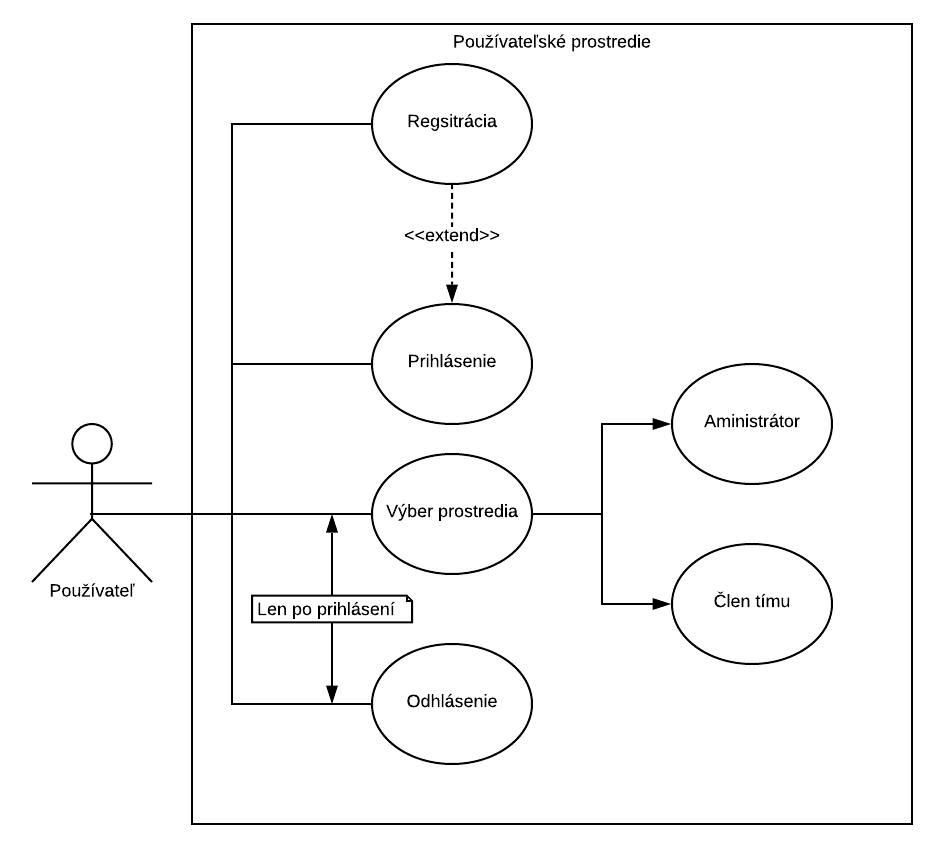
\includegraphics[scale=0.50]{img/DP_use_case_pouzivatel.png}
    \caption{Use case diagram pre používateľské prostredie}
    \label{fig:use_case_pozivatel}
\end{figure}

\indent Druhý diagram - Obr.~\ref{fig:use_case_administrator} nám ilustruje prípady použitia ak používateľ vybral možnosť prihlásiť sa ako administrátor, prípadne ak sa člen tímu prepol do admnistrátorského rozhrania. Administrátor teraz môže buť spravovať svoje tímy alebo vytvoriť nový tím.

\begin{figure}[H]
    \centering
    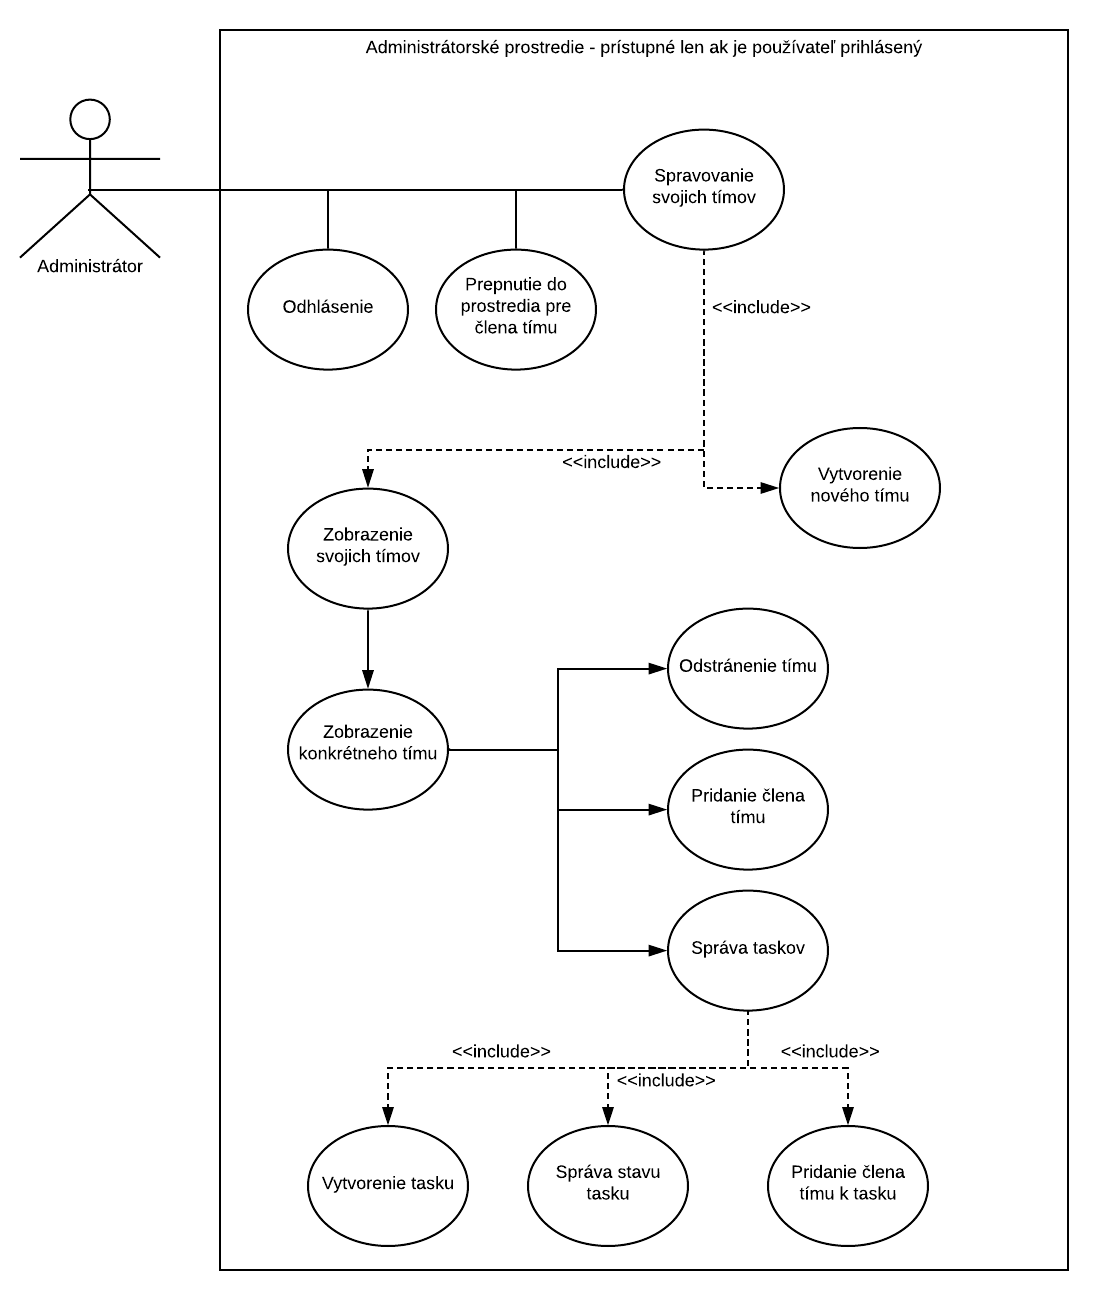
\includegraphics[scale=0.45]{img/DP_use_case_administrator.png}
    \caption{Use case diagram pre administrátorské prostredie}
    \label{fig:use_case_administrator}
\end{figure}

\indent Posledný diagram prípadov použitia - Obr.~\ref{fig:use_case_clen_timu} nám ilustruje, ako môže používateľ používať systém, ak si vybral možnosť prihlásiť sa ako člen tímu alebo sa prepol z admnistrátorského rozhrania do rozhrania člena tímu. Tu má používateľ na výber viacero možností, čo môže v aplikácii vykonať.

\begin{figure}[H]
    \centering
    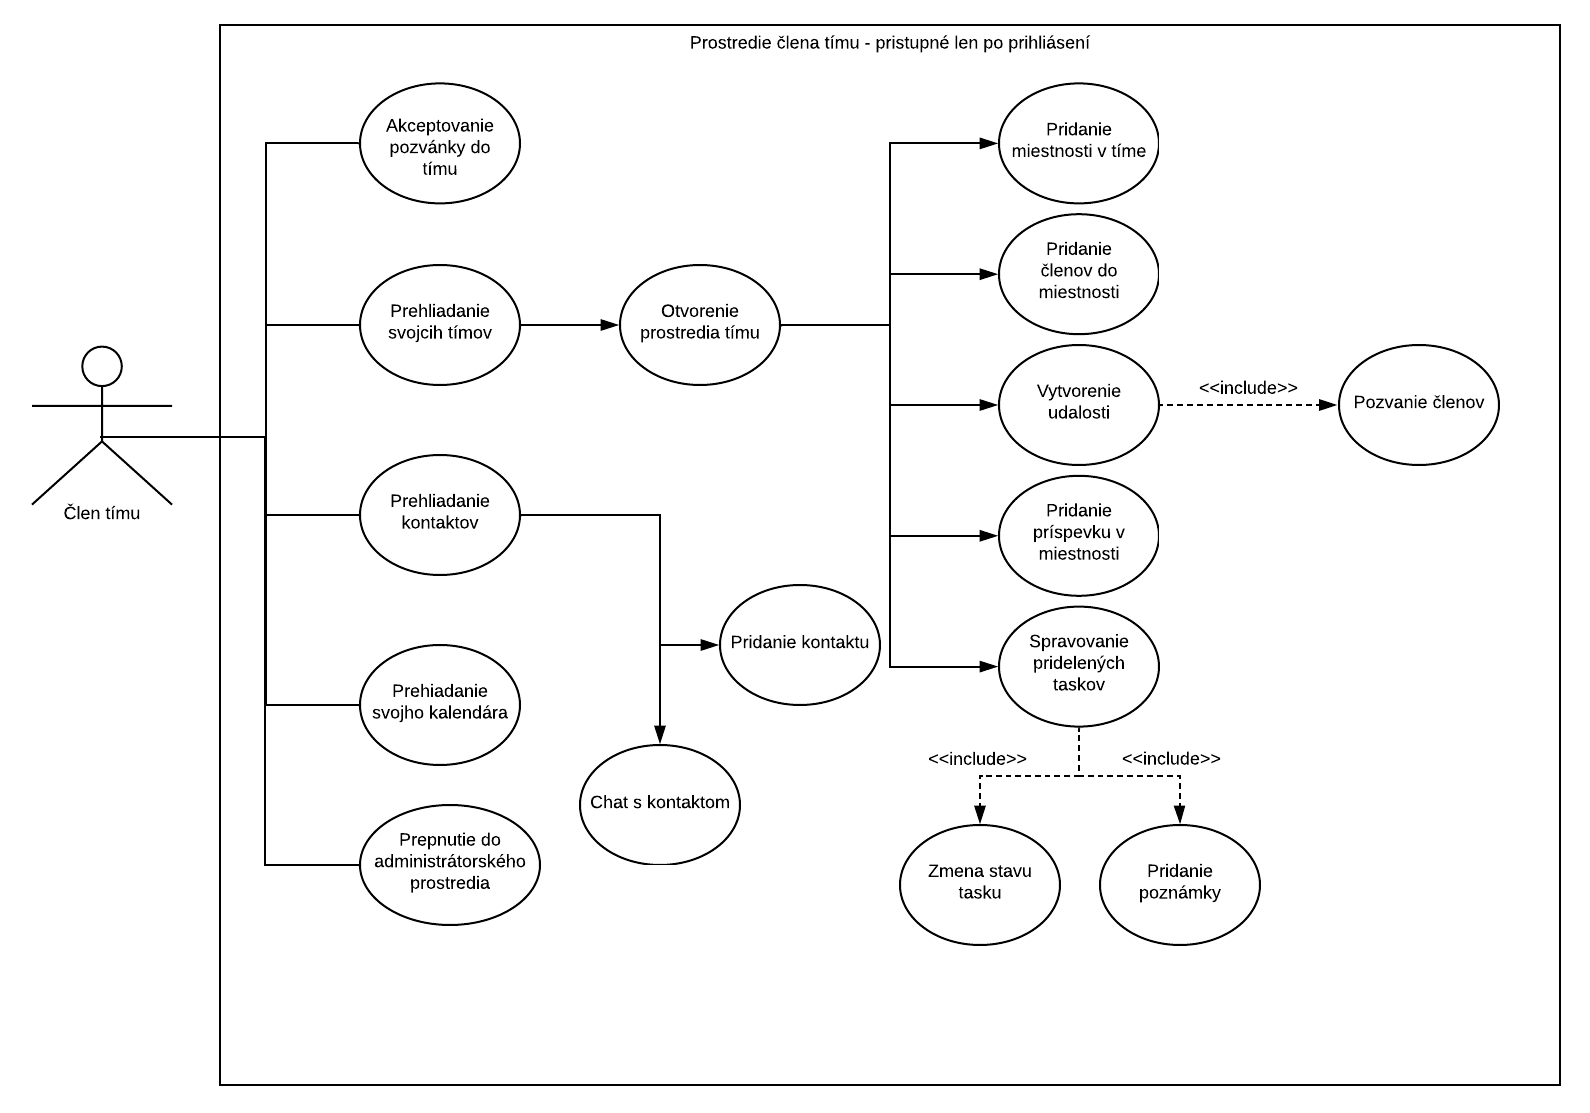
\includegraphics[scale=0.20]{img/DP_use_case_clen_timu.png}
    \caption{Use case diagram prostredia člena tímu}
    \label{fig:use_case_clen_timu}
\end{figure}

\subsubsection{Sekvenčné diagramy}
\indent Nasledujúce diagramy budú asi najpoužívanejšie pri implementácii aplikácie, nakoľko sekvenčné diagramy nám ukazujú interakcie medzi komponentami v systéme.
\newline
\newline
\textbf{Prihlásenie a registrácia} \newline
\indent Na Obr.~\ref{fig:seq_login} môžeme vidieť komunikáciu jednotlivých komponentov pri prihlásení alebo registrácii do aplikácie. Na základe výberu používateľa, či sa chce prihlásiť alebo registrovať, sa mu zobrazí príslušná stránka. Pri prihláseni sa a po vyplnení údajov sa tieto údaje pošlú na server, ktorý v online databáze skontroluje daný email či používateľ existuje. Ak existuje, skontroluje aj heslo. Ak sú oba údaje správne, server vytvorí autorizačný token s určitou platnosťou a pošle ho kientovi. Na strane klienta sa potom vytvorí lokálna databáza, ktorá si hneď z online databázy stiahne všetky dáta a aplikácia tu začína pracovať len s lokálnou databázou. 

\begin{figure}[H]
    \centering
    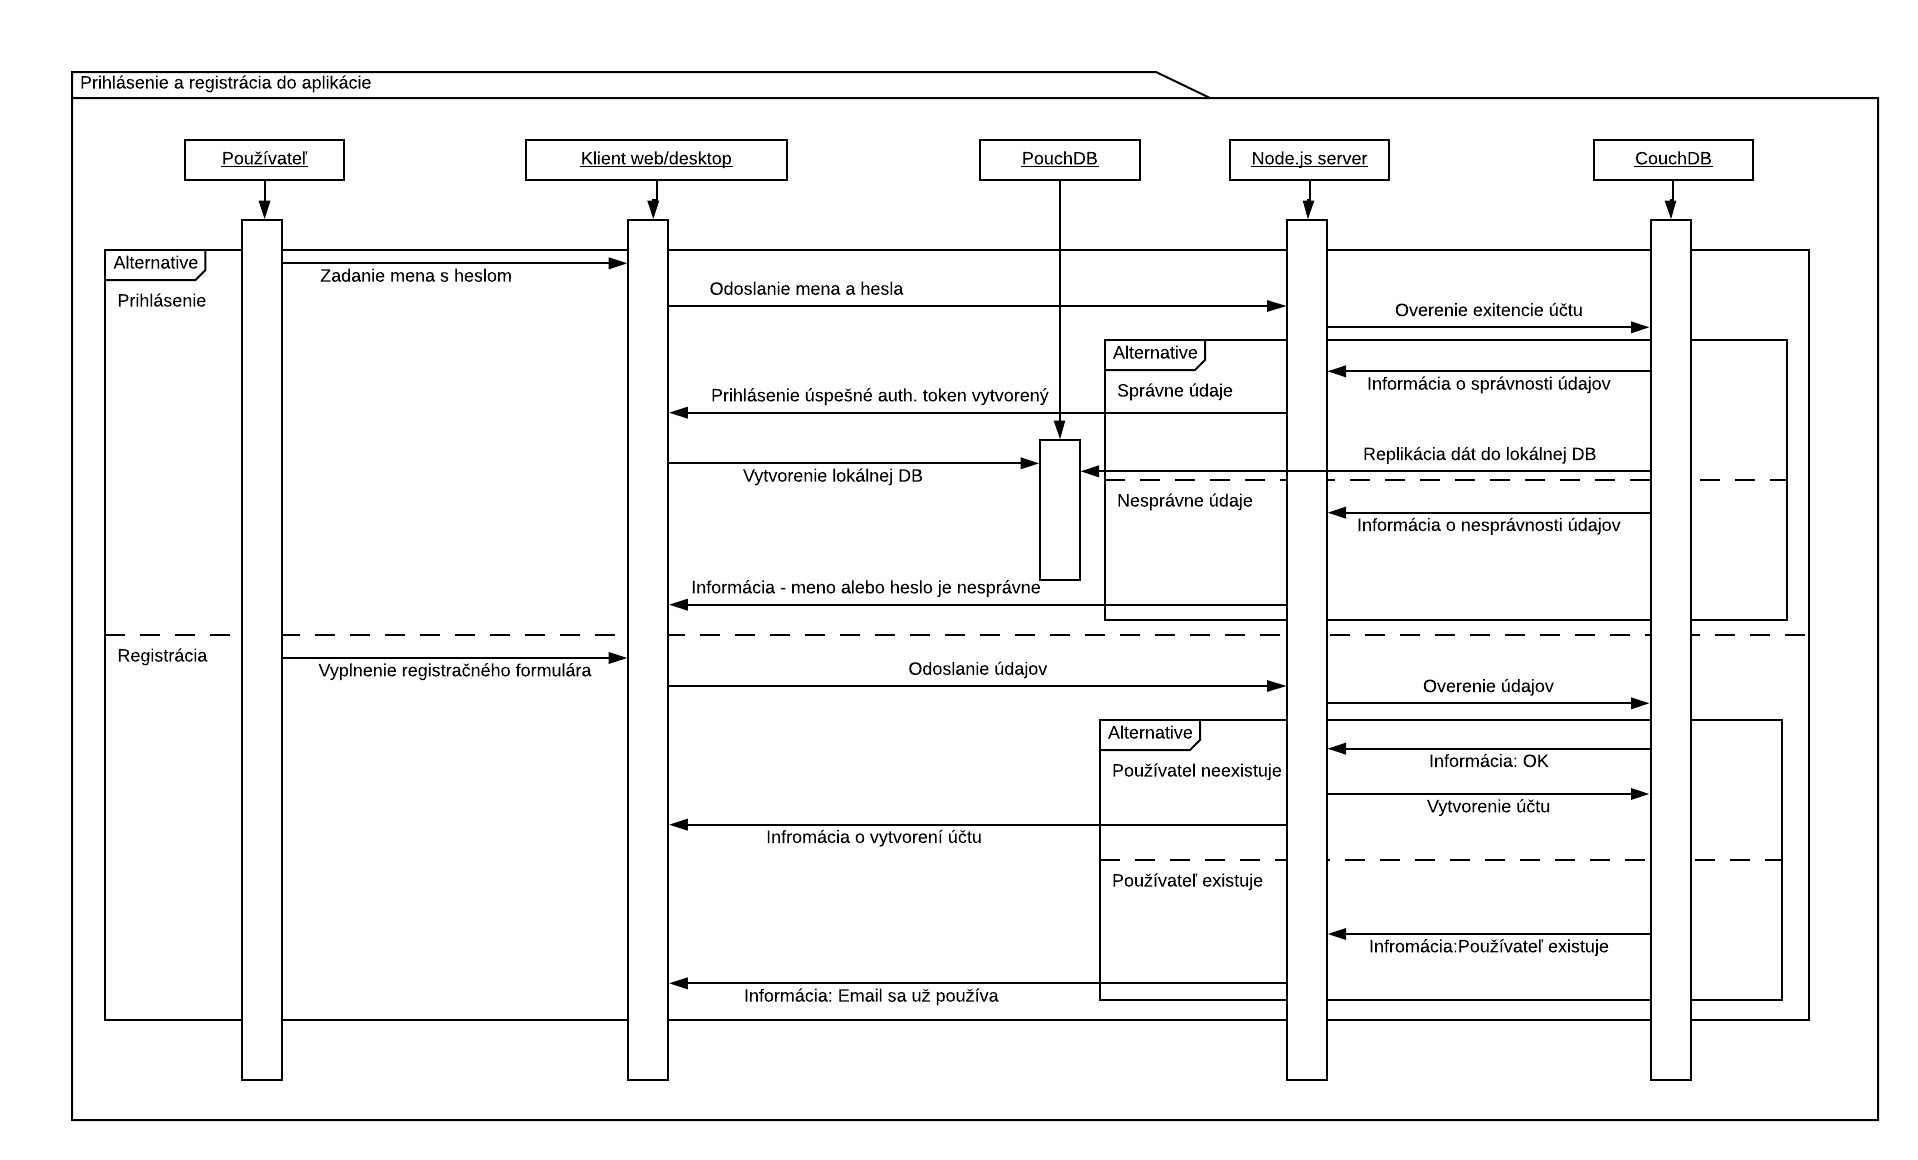
\includegraphics[scale=0.50]{img/Seq_login_register.png}
    \caption{Sekvenčný diagram prihlásenia a registrácie}
    \label{fig:seq_login}
\end{figure}

\indent Pri registrácii funguje systém podobne. Po vyplnení údajov sa údaje pošlú na server, ktorý overí či daný email sa už nepoužíva. Ak sa nepoužíva, tak sa do databázy uloží nový používateľ a na stranu klienta je odoslaná správa o úspešenej registrácii. 
\newpage
\noindent\textbf{Komunikácia komponentov v aplikácii po prihlásení} \newline
\indent Diagram Obr.~\ref{fig:seq_com} nám znázorňuje, ako budú jednotlivé komponenty v aplikácii medzi sebou komunikovať po prihlásení do aplikácie.
\begin{figure}[H]
    \centering
    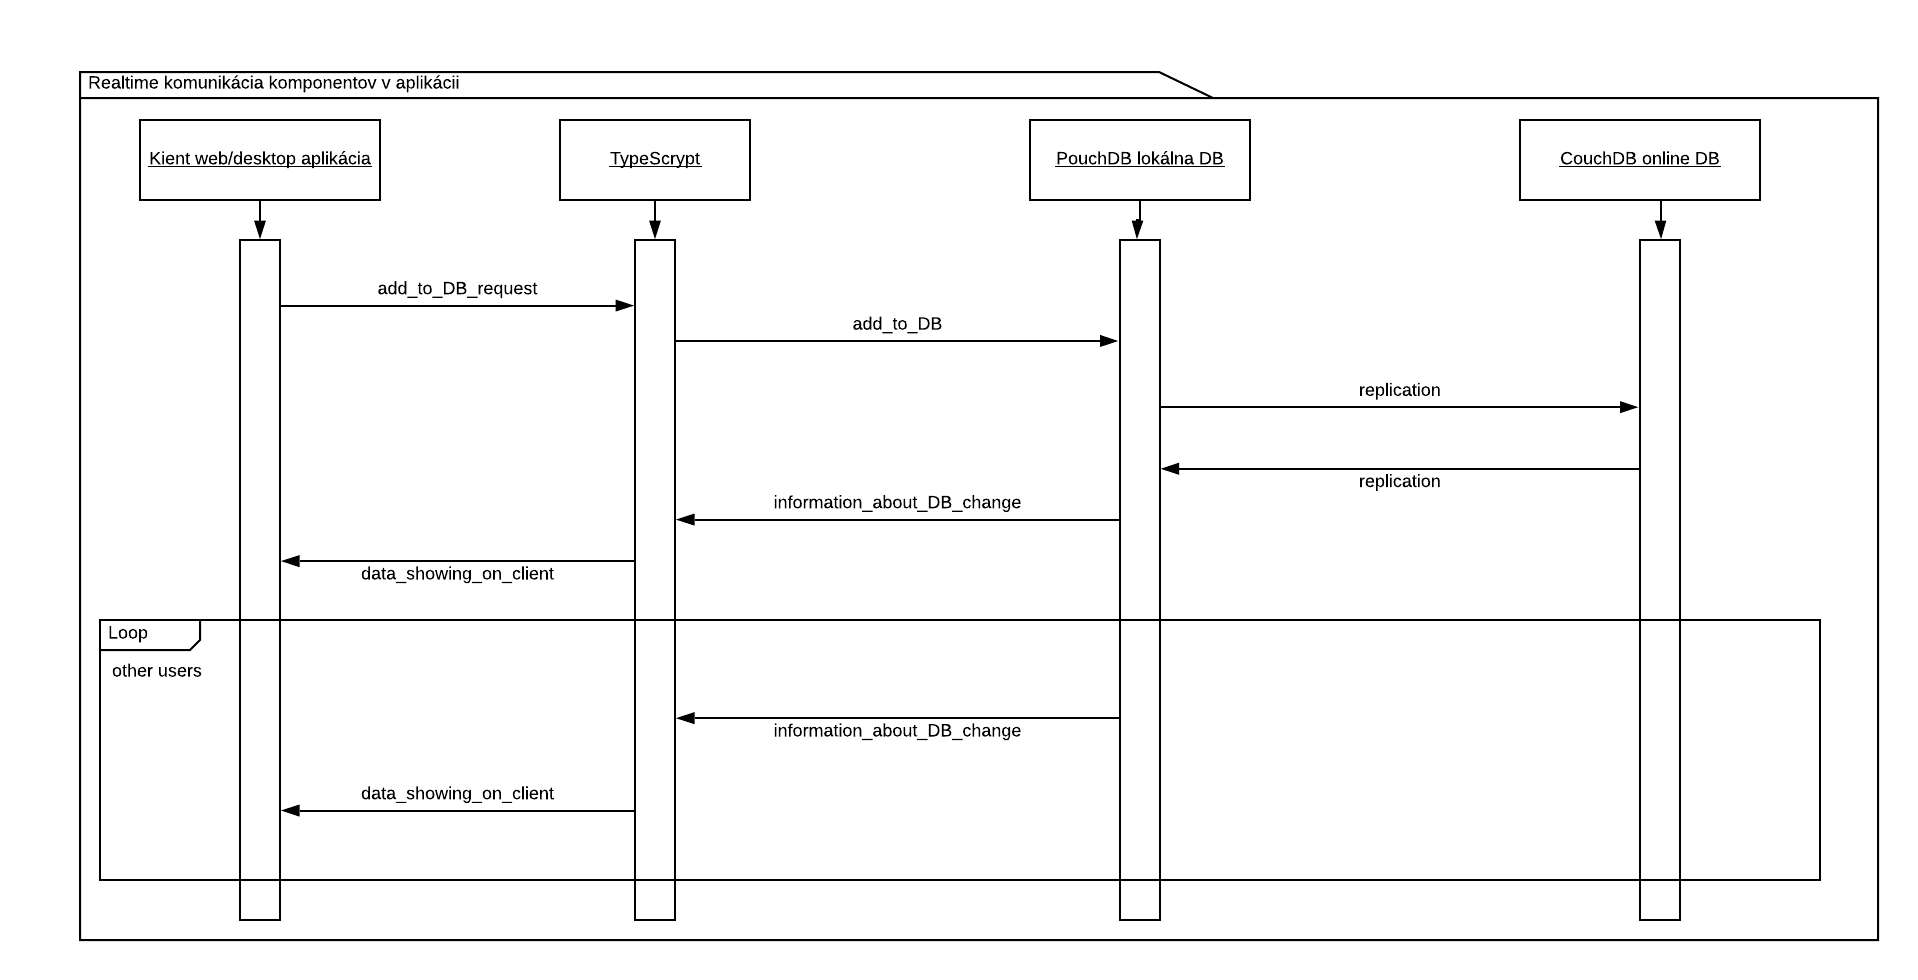
\includegraphics[scale=0.50]{img/seq_tim.png}
    \caption{Sekvenčný diagram komunikácie komponentov v aplikácii}
    \label{fig:seq_com}
\end{figure}

\indent Celá komunikácia je založená na http protokole. Na diagrame môžeme vidieť, že ak niektorý používateľ vytvorí tím, udalosť, úlohu alebo napíše správu, tak je vytvorená žiadosť na pridanie do databázy. Pridanie do databázy je realizované tak, že najskôr sú dáta pridané do lokálnej databázy PouchDB a ak má zariadenie, na ktorom beží aplikácia prístup na internet, sú tieto dáta hneď zreplikované do online databázy. Ak prístup na internet nie je, tak sú dáta zatiaľ uložené len v lokálnej databáze do doby, kým zariadenie nezíska prístup na internet. Ostatným používateľom je potom odoslaná informácia, že na strane databázy prišlo k zmene a ich dáta, ktoré sa v klientovi zobrazujú sú aktualizované na základe nových dát v databáze.  

\subsection{Databázový model CouchDB}
\indent Po analýze viacerých možností sme sa v našom zadaní rozhodli nepoužiť štandardnú SQL databázu. Toto má za následok to, že sa nedá modelovať databáza cez štandarné ERD diagramy. CouchDB je databáza založená nie na tabuľkách, ale na JSON dokumentoch. Hoci si naša aplikácia bude vyžadovať viac špecifických objektov pre jednotlivé záznamy do databázy, tieto objekty nebudú zložité. Jedná sa prevažne o objekty zložené z viacerých jednoduchých dátových hodnôt typu string, integer, date. Tieto objekty bude potrebné vytvoriť ako na strane servera v JavaScripte, tak aj na strane frontendu v TypeScripte. Návrh jednotlivých objektov môžeme vidieť nižšie spolu s ich neskoršou reprezentáciou v JSON dokumentoch na strane CouchDB. Rozdiely oproti návrhu a ich neskoršou reprezentáciou sú spôsobené potrebou zmeny pri implementácii aplikácie kvôli zjednodušeniu jej behu. 

\textbf{Používateľ:}
\indent\begin{itemize}
    \item základné údaje meno priezvisko heslo mail
    \item popis používateľa
    \item kontakty 
    \item miestnosti
    \item kalendár 
\end{itemize}

\begin{figure}[H]
    \centering
    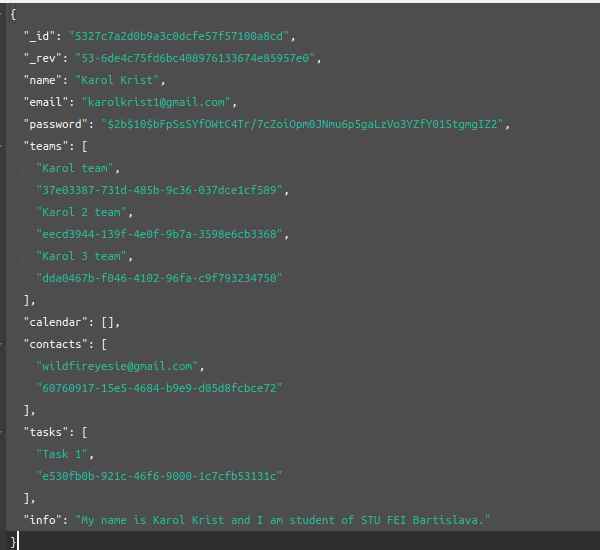
\includegraphics[scale=0.50]{img/imp/db_user.png}
    \caption{JSON dokument používateľa v Couchdb}
    \label{fig:db_user}
\end{figure}

\textbf{Udalosť:}
\indent\begin{itemize}
    \item názov
    \item tím 
    \item začiatok
    \item koniec
    \item popis 
\end{itemize}

\begin{figure}[H]
    \centering
    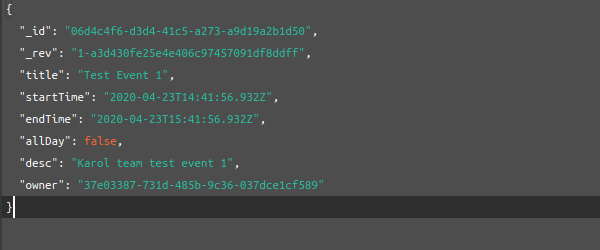
\includegraphics[scale=0.50]{img/imp/db_event.png}
    \caption{JSON dokument udalosti v Couchdb}
    \label{fig:db_event}
\end{figure}

\textbf{Tím:}
\indent\begin{itemize}
    \item názov
    \item admin 
    \item členovia  
    \item miestnosti 
    \item udalosti 
    \item úlohy 
\end{itemize}

\begin{figure}[H]
    \centering
    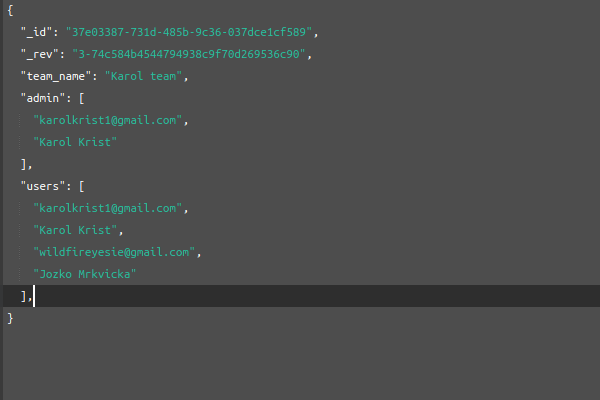
\includegraphics[scale=0.50]{img/imp/db_team.png}
    \caption{JSON dokument tímu v Couchdb}
    \label{fig:db_team}
\end{figure}

\textbf{Miestnosť:}
\indent\begin{itemize}
    \item názov
    \item členovia 
    \item príspevky 
\end{itemize}

\begin{figure}[H]
    \centering
    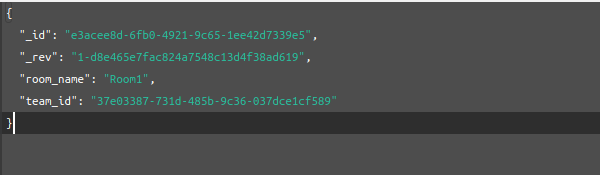
\includegraphics[scale=0.50]{img/imp/db_room.png}
    \caption{JSON dokument miestnosti v Couchdb}
    \label{fig:db_room}
\end{figure}

\textbf{Príspevok:}
\indent\begin{itemize}
    \item text
    \item autor
    \item čas pridania
    \item miestnosť
\end{itemize}

\begin{figure}[H]
    \centering
    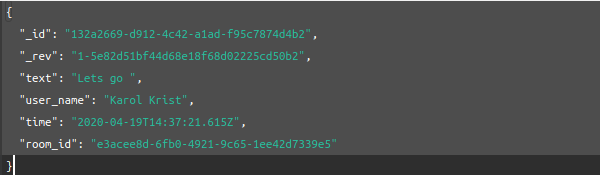
\includegraphics[scale=0.50]{img/imp/db_feed.png}
    \caption{JSON dokument príspevku v miestnosti v Couchdb}
    \label{fig:db_feed}
\end{figure}

\textbf{Správa:}
\indent\begin{itemize}
    \item text
    \item autor 
    \item komu
    \item čas odoslania
\end{itemize}

\begin{figure}[H]
    \centering
    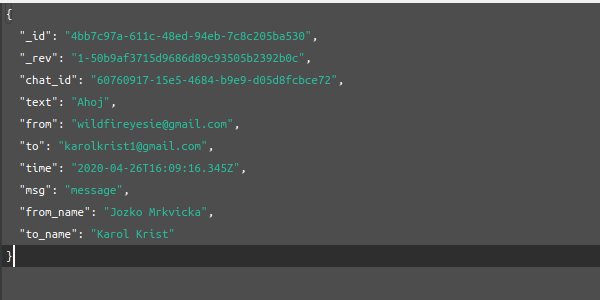
\includegraphics[scale=0.50]{img/imp/db_message.png}
    \caption{JSON dokument správy v Couchdb}
    \label{fig:db_message}
\end{figure}

\textbf{Úloha:}
\indent\begin{itemize}
    \item názov
    \item vedúci úlohy
    \item text
    \item tím
    \item pridelení používatelia
    \item stav úlohy
    \item komentáre
\end{itemize}

\begin{figure}[H]
    \centering
    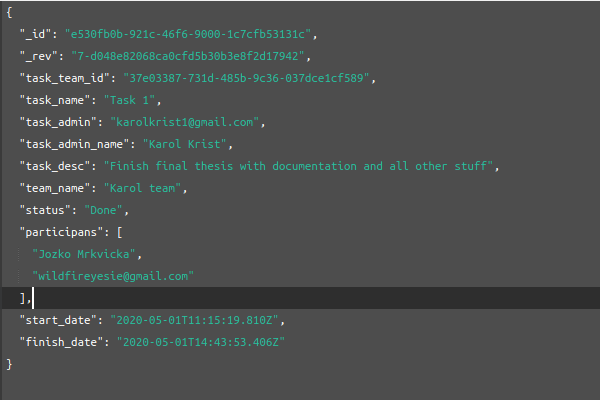
\includegraphics[scale=0.50]{img/imp/db_task.png}
    \caption{JSON dokument úlohy v Couchdb}
    \label{fig:db_task}
\end{figure}

\textbf{Komentár:}
\indent\begin{itemize}
    \item text
    \item autor
    \item čas pridania
    \item úloha
\end{itemize} 

\begin{figure}[H]
    \centering
    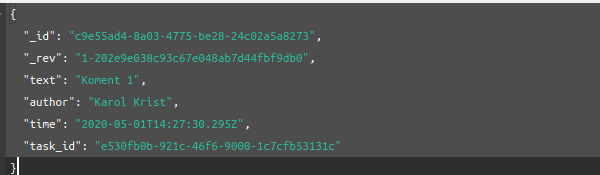
\includegraphics[scale=0.50]{img/imp/db_comment.png}
    \caption{JSON dokument komentáru úlohy v Couchdb}
    \label{fig:db_comment}
\end{figure}

\section{Implementácia aplikácie}
\indent Po vypracovaní kompletného návrhu sme začali s implementáciou. Tá sa dala rozvrhnúť na viac fáz podľa toho, ako sme postupne implementovali aplikáciu. Začali sme s implementáciou prihlasovacieho a registračného systému. Po dokonční tejto časti sme prešli do implementácie zobrazenia aplikácie po prihlásení používateľa. Tu sme implementovali časť aplikácie, kde sú zobrazené informácie o aktuálne prihlásenom používateľovi, tímy, ktorých je členom, jeho kalendár, v ktorom sú zobrazené udalosti jeho tímov, stránka všetkých jeho úloh zo všetkých tímov a stránka jeho kontaktov. Po implementovaní tejto časti sme prešli na implementáciu vytvárania a správy tímov. Následne sme implementovali jednotlivé funkcie, ktoré vie vykonávať, či už admin tímu alebo člen tímu vo vybranom tíme. Sem patrí vytváranie a správa miestností, úloh a udalostí vo vybranom tíme. Predposlednou časťou, ktorou sme sa zaoberali bolo vytvorenie chatu medzi používateľmi, ktorých máme v kontaktoch. Poslednou časťou bolo vyladenie potencionálnych problémov a celkový dizajn aplikácie nakoľko doteraz sme implementovali hlavne funkcionálne časti aplikácie a dizajn sme nechávali na koniec. Všetky časti, až na poslednú, sa dajú ešte rozdeliť na implemetáciu back-end časti a front-end časti. Tieto dve časti sme vždy implementovali súčasne, aby sme si vždy otestovali požadovanú funkčnosť. Finálnym krokom bol export aplikácie pomocou Elektronu na desktopovú aplikáciu. Nižšie si teraz prejdeme postupne všetky fázy implementácie a podrobne si rozoberieme ako sme jednotlivé časti implementovali.

\subsection{Prihlasovanie a registrácia}
\indent Medzi nefunkcionálnymi požiadavkami sme spomínali fungovanie aplikácie aj v offline režime. Táto časť aplikácie bola ale implemetovaná tak, aby ako jediná vyžadovala pripojenie na internet. Je to samozrejmé z dôvodu, že na získanie dát z online databázy CouchDB a ich zreplikovanie do lokálnej databázy PouchDB vyžaduje pripojenie na internet. Popíšeme si najskôr, ako sme implementovali back-end tejto časti a potom font-end.

\indent Na implementáciu back-endu prihlásenia a registrácie sme využili Node.js server, ktorý sa prípája na online databázu. Na Obr. ~\ref{fig:register_back} môžeme vidieť implementáciu funkcie na registráciu používateľa. Po odoslaní vyžadovaných dát používateľom z registračnej stránky sa z requestu - req vytiahnu dáta email, meno a heslo. Prvé, čo sa vo funkcii vykoná, je overenie, či boli zaslané všetky tri údaje. Ak nie, server vráti status 400 so správou, že používateľ nezadal všetky potrebné údaje. Ak boli zaslané všetky tri, tak sa vytvorí selektor do databázy, kde sa overuje zadaný email. Ak sa v databáze už nachádza vytvorený používateľ so zaslaným emailom, tak server vráti opäť status 400 so správou, že používateľ s týmto emailom už existuje. Rozhodli sme sa overovať len na základe emailu, pretože sa môže stať, že dvaja používatelia majú rovnaké meno. Ak v databáze takýto používateľ neexistuje, tak sa najskôr zašifruje heslo pomocou prídavnej knižnice do Node.js bcrypt. Následne sa už len vytvoria potrebné dodatočné záznamy, ktoré JSON dokument používateľa potrebuje - polia tímov, udalostí, kontaktov, úloh a prázdny popis používateľa a tento údaj sa pomocou prídavnej knižnice na prácu s CouchDB nano pridá do databázy pomocou funkcie insert.
\begin{figure}[H]
    \centering
    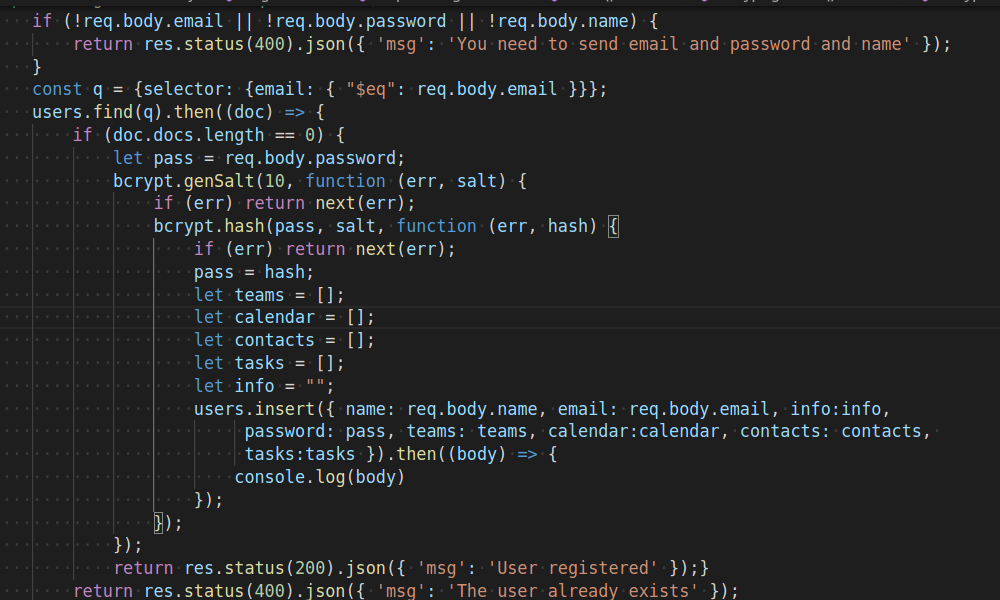
\includegraphics[scale=0.45]{img/imp/register_back.png}
    \caption{Funkcia register na strane back-endu}
    \label{fig:register_back}
\end{figure}

\indent Na Obr. ~\ref{fig:login_back} je kód funkcie na prihlásenie. Podobne, ako pri registračnej funkcii, sa najskôr overí, či používateľ zadal všetky potrebné údaje. Následne sa overí, či zadaný používateľ je v databáze vytvorený. Ak je, tak sa z databázy vytiahne celý jeho JSON dokument a overí sa či bolo zadané správne heslo.

\begin{figure}[H]
    \centering
    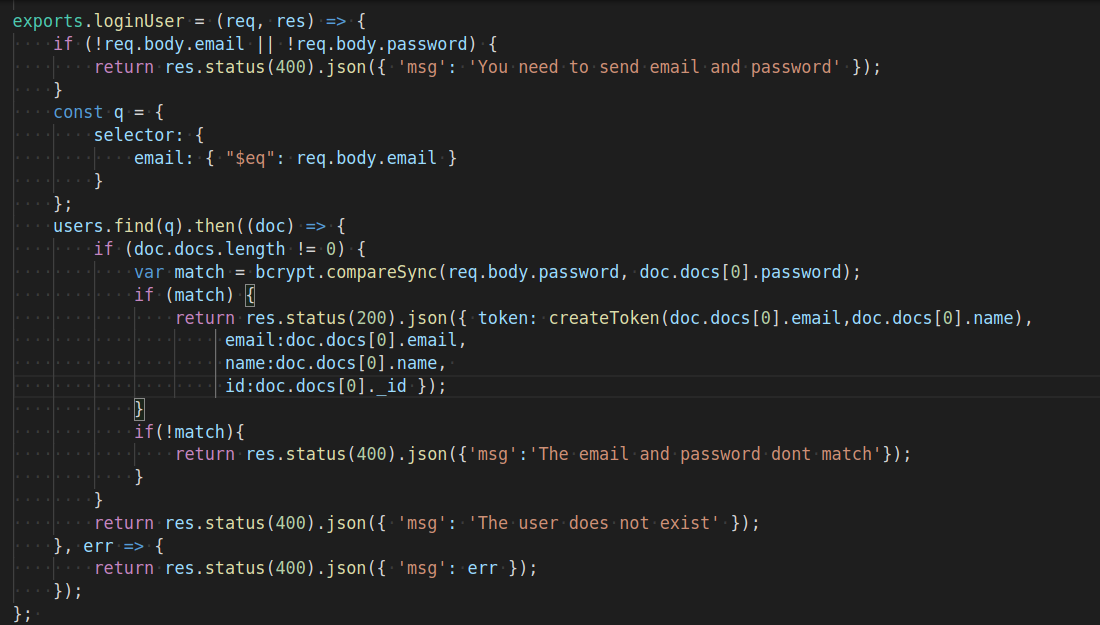
\includegraphics[scale=0.40]{img/imp/login_back.png}
    \caption{Funkcia login na strane back-endu}
    \label{fig:login_back}
\end{figure}

\indent Ak je všetko v poriadku, vytvorí sa pomocou funkcie createToken jsonwebtoken. Kód tejto funkcie môžeme vidieť na Obr. ~\ref{fig:jwt}. Na vytvorenie tokena je potrebná dodatočná knižnica jsonwebtoken. V tokene je uložené meno a email prihláseného používateľa, takzvané "JWT tajomstvo", čo je string, podľa ktorého sa token šifruje a dĺžka platnosti tokena - v našom prípade 24 hodín. Po vypršaní tokena sa automaticky používateľ odhlási a musí byť prihlásený na novo. 

\begin{figure}[H]
    \centering
    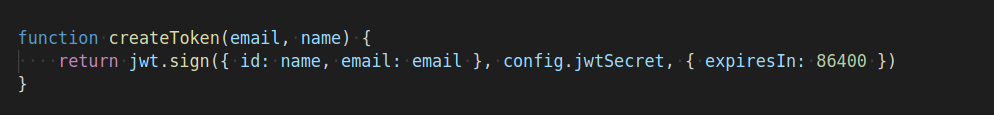
\includegraphics[scale=0.42]{img/imp/jwt.png}
    \caption{Vytvorenie JWT tokenu}
    \label{fig:jwt}
\end{figure}

\indent Na strane front-endu sme ako základ implementovali tiež dve funkcie login a register, ktoré len z formulára vytiahnu zadané údaje a pošlú ich na adresu servera s volaním smerovania, aké sme nastavili pre login a register. Na volanie adries servera sme použili dodatočné moduly pre Angular a Ionic HTTPClient a na prácu s JWT tokenom JwtHelperService. Funkcie login a register môžeme vidieť na Obr ~\ref{fig:login_front}. 

\begin{figure}[H]
    \centering
    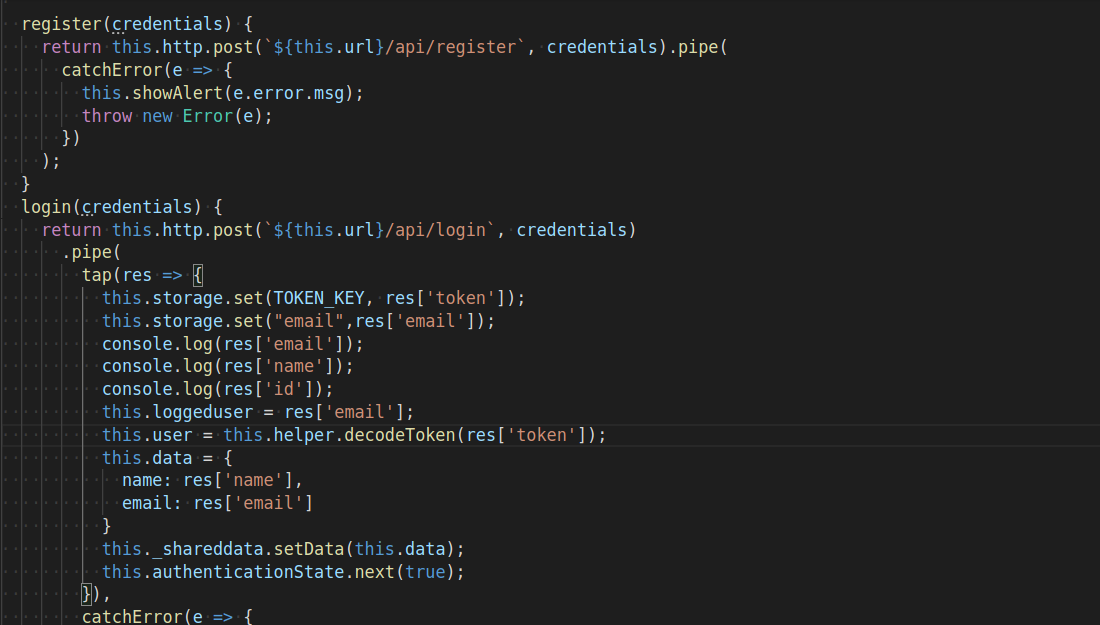
\includegraphics[scale=0.40]{img/imp/login_front.png}
    \caption{Prihlásenie a registrácia na strane front-endu}
    \label{fig:login_front}
\end{figure}

\indent Na strane font-endu sme implementovali ešte niekoľko ďalších potrebných funkcií. Samozrejmá je funkcia na odhlásenie používateľa, kde sa len zmazal JWT token. Tiež dôležitou funkciou bola funkcia na overenie platnosti tokena. Pri prihlásení sa token uložil do lokálnej pamäte. Pri každom načítaní, niektorej z ďalej vytvorených stránok sa volá funkcia checkToken (Obr. ~\ref{fig:checkjwt} ). Tu sa pomocou vyššie spomenutej knižnice na prácu s JWT tokenom overí platnosť tokena. Ak nie je platný, tak sa nastaví autorizačný stav na false a používateľ pri otvorení novej stránky alebo obnovení aktuálnej bude automaticky odhlásený a presmerovaný na prihlasovaciu stránku. 

\begin{figure}[H]
    \centering
    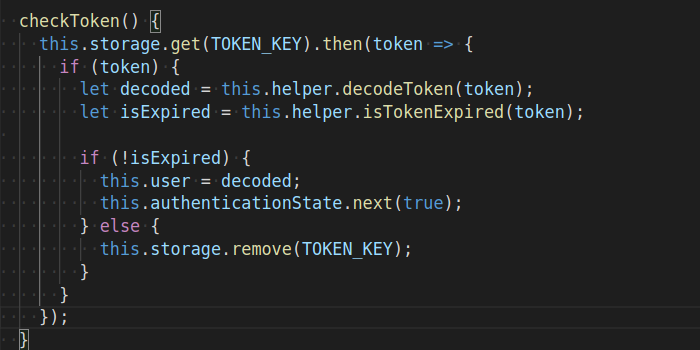
\includegraphics[scale=0.50]{img/imp/checkjwt.png}
    \caption{Overenie platnosti JWT tokenu}
    \label{fig:checkjwt}
\end{figure}

\subsection{Stránka prihláseného používateľa}
\indent Po prihlásení sa používateľovi zobrazí stránka s postranným menu, kde si vie zvoliť z 5 možností - profil, tímy, kalendár, úlohy a kontakty, plus sa tu nachádza možnosť odhlásenia. Hneď po načítaní tejto stránky sa online databáza CouchDB zreplikuje do lokálnej databázy PouchDB a nastaví sa takzvané počúvanie databázy na live zmeny, čo umožní v reálnom čase meniť zobrazené dáta hneď po ich editácii, pridaní alebo zmazaní z databázy. Toto nastavenie sa realizuje pomocou vstavanej funkcie knižnice pouchdb changes() (Obr. ~\ref{fig:db_change}). 

\begin{figure}[H]
    \centering
    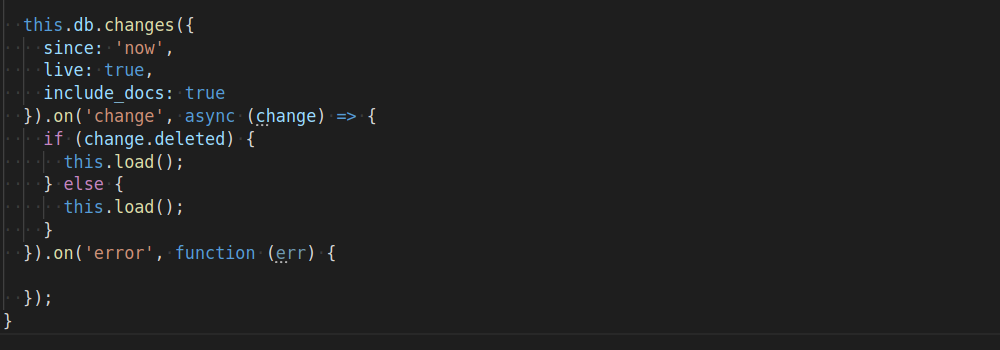
\includegraphics[scale=0.45]{img/imp/db_change.png}
    \caption{Nastavenie na live počúvanie zmien databázy}
    \label{fig:db_change}
\end{figure}

\indent Táto časť bola jednoduchá. Prvým krokom bolo vytvorenie spojenia s lokálnou databázou. Spojenie sme nadviazali pomocou prídavného modulu pre Angular pouchdb. Po vytvorení spojenia sa načítajú dáta aktuálne prihláseného používateľa. Tieto údaje sú potom podľa výberu v menu distribuované pomocou nami vytvorenej service sharreddata medzi jednotlivými stránkami, ktoré ich zobrazujú. Service sharreddata pozostáva len z premenných, do ktorých ukladáme dáta z DB a z ich getterov a setterov. Toto načítanie dát z databázy a uloženie do sharreddata je na Obr. ~\ref{fig:loged_back}.  

\begin{figure}[H]
    \centering
    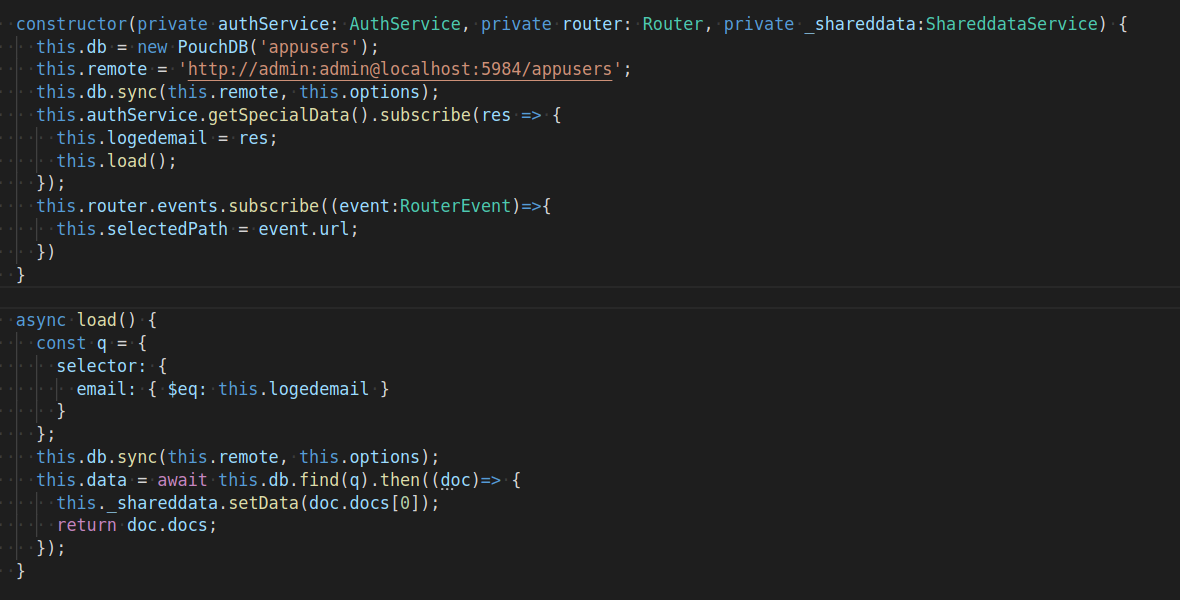
\includegraphics[scale=0.38]{img/imp/loged_user_back.png}
    \caption{Načítanie dát prihláseného používatela}
    \label{fig:loged_back}
\end{figure}

\indent Zobrazenie dát na stránke sme následne realizovali podľa potreby. Stránka profilu len zobrala dopredu vytiahnuté dáta z DB o používateľovi a zobrazila ich. Na zobrazenie tímov, ktorých členom je prihlásený používateľ sme použili tabuľkové rozloženie a funkciu Angularu ngFor. Táto funkcia prechádza polom tímov a vykresľuje dáta každého prvku v poli podľa predlohy. Podobným princípom sme vytvorili aj zobrazenie kontaktov prihláseného používatela. Ukážka kódu tohto zobrazenia je na Obr. ~\ref{fig:teams}

\begin{figure}[H]
    \centering
    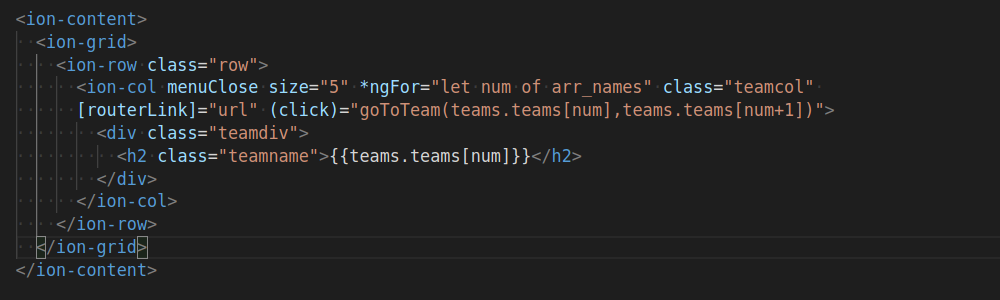
\includegraphics[scale=0.45]{img/imp/teams.png}
    \caption{Zobrazenie používateľových tímov}
    \label{fig:teams}
\end{figure}

\indent Na vykreslenie kalendára s udalosťami sme použili prídavný modul Ionicu ionic2-calendar. Tento modul nám umožnil použiť html element calendar (Obr. ~\ref{fig:calendar}), ktorý pekne vykresľuje kalendár s možnosťou prepínania zobrazenia na zobrazenie jednotlivých dní alebo zobrazenie mesiaca, prípadne týždňa. Tak isto sa veľmi jednoducho pracuje so zobrazením udalostí, nakoľko stačí do elementu poslať pole udalostí, ktoré sú vo formáte json, čo nám uľahčilo prácu, nakoľko nebolo potrebné vytiahnuté dáta z databázy upravovať. Jediný údaj potrebný upraviť bol dátum a čas, nakoľko ten sa do databázy ukladal ako String a element kalendár očakával dátový typ Date.

\begin{figure}[H]
    \centering
    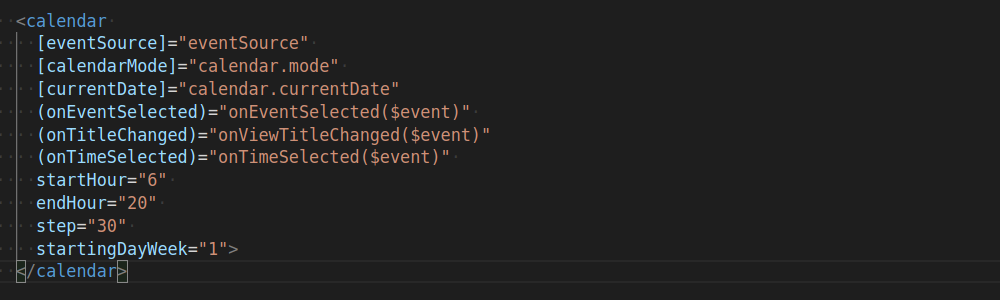
\includegraphics[scale=0.45]{img/imp/calendar_user.png}
    \caption{Použitie html elementu calendar}
    \label{fig:calendar}
\end{figure}

\subsection{Stránka vybraného tímu}
\indent Keď používateľ na stránke po prihlásení otvoril stránku s jeho tímami, má možnosť na niektorý z jeho tímov kliknúť. Po kliknutí sa mu otvorí stránka tímu, ktorá pozostáva z viacerých možností. Základom stránky je postranné menu, kde sú zobrazené vytvorené miestnosti v teame a vytvorené úlohy v teame. Taktiež tu je možnosť prezrieť si kalendár tímu a stránku s členmi tímu, kde sú zobrazené profily členov tímu a je tu taktiež možnosť pridania používateľa do kontaktov. Administrátor, respektíve vedúci tímu má navyše možnosť pridávania členov do tímu a vytváranie prípadne odstránenie udalostí v tímovom kalendári. Vytváranie miestností a úloh je umožnené všetkým členom tímu. 

\indent Implementáciu tejto časti sme začali implementovaním funkcie pre administrátora tímu na pridanie členov do tímu a následne ich zobrazenie na stránke členov. Pridávanie členov sme zrealizovali pomocou vyskakovacích alert okien, kde administrátor zadá email používateľa, ktorého chce pridať. Kód implementácie vyskakovacieho okna môžeme vidieť na Obr.  ~\ref{fig:add_user_alert}. Následne sa tento email použije na vyhľadanie v databáze. Ak je používateľ s tímto emailom nájdený, je pridaný do tímu a administrátor je o tom  informovaný vyskakovacím oknom. Ak sa tento email nenašiel so žiadnym používateľom, opäť vyskočí informácia o tom, že daný používateľ neexistuje. Samotnú stránku členov tímu sme implementovali rovnako ako stránku kontaktov pri úvodnej stránke po prihlásení. 

\begin{figure}[H]
    \centering
    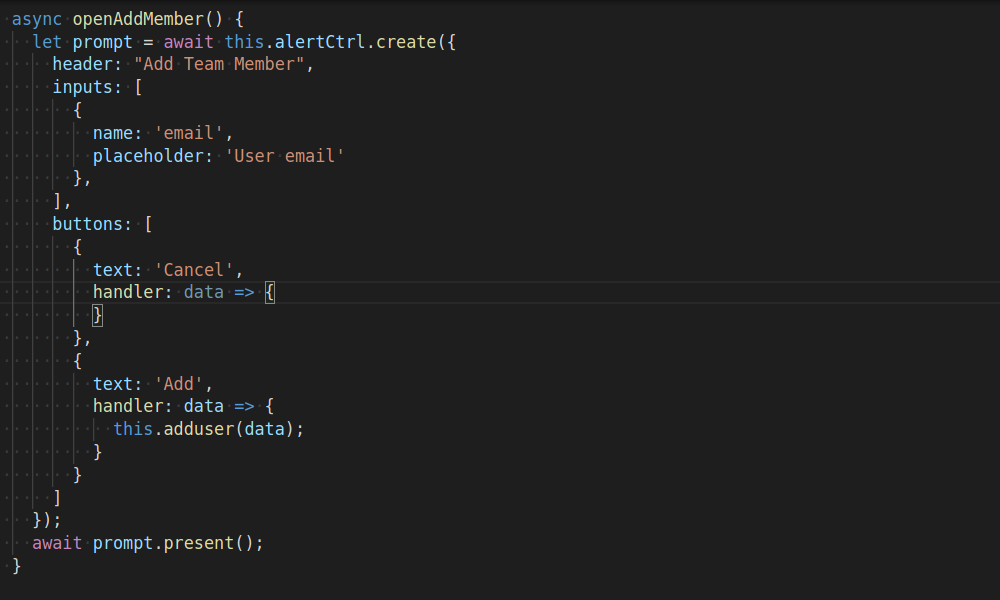
\includegraphics[scale=0.45]{img/imp/add_user_alert.png}
    \caption{Implementácia vyskakovacieho okna na pridanie člena tímu}
    \label{fig:add_user_alert}
\end{figure}

\indent Ďalšou časťou, ktorú sme implementovali bol kalendár a pridávanie udalostí. Kalendár sme implementovali rovnako ako pri kalendári používateľa. Jediným rozdielom bolo načítanie dát. Tu sme načítavali udalosti len tímu, v ktorom sa nachádzame. Pridávanie udalostí sme implementovali pomocou rozbalovacieho okna, kde po kliknutí na tlačidlo pridanie udalosti sa nám rozbalí formulár, do ktorého treba zadať názov udalosti, jej popis, čas od kedy do kedy bude udalosť prebiehať, prípadne vybrať možnosť udalosť na celý deň. V tomto prípade sa do času začiatku uloži vybraný deň a čas 7:00 ráno a do času konca sa uloži vybraný deň konca a čas 22:00. 

\indent V implementácii tímovej časti sme ďalej pokračovali vytvorením funkcionality miestností. Tu sme najkôr implementovali možnosť vytvorenia miestnosti. Toto sme realizovali podobne ako pridanie člena do tímu pomocou vyskakovacieho okna, kde sa zadal názov miestnosti. Následne sa vytvorená miestnosť zobrazila v bočnom menu. Po kliknutí na názov miestnosti v menu sa otvorí stránka miestnosti, na ktorej sa zobrazia pridané príspevky a možnosť pridať nový príspevok. Zobrazenie príspevkov sme realizovali pomocou vyššie spomínanej funkcie Angularu ngFor, ktorá pre každý príspevok vytiahnutý z databázy vytvorila zobrazenie dát príspevku podľa predlohy. Na spodku stránky sme implementovali pridanie príspevku. To pozostáva z jednoduchého elementu textarea, ktorý sa po kliknutí naň jemne zväčší a používateľ môže napísať správu príspevku. Po stlačení tlačidla enter sa potom príspevok vytvorí pod menom prihláseného používateľa a čas pridania sa nastaví na aktuálny čas. Takto vytvorený príspevok sa pošle do databázy. Pomocou na začiatku spomínanej funkcie changes() sa hneď príspevok zobrazí všetkým online používateľom. 

\indent Poslednou funkcionalitou, ktorú sme v tejto časti implemetovali bolo vytváranie, zobrazenie a správa úloh. V postrannom menu sme implementovali tlačidlo na pridanie úlohy. Toto sme tiež implementovali pomocou vyskakovacieho okna, kde používateľ zadá názov a popis úlohy. Následne je úloha vytvorená a zobrazí sa v postrannom menu, kde je možné na ňu kliknúť. Po kliknutí sa zobrazí stránka úlohy, kde sú zobrazené jej údaje, komentáre od používateľov a možnosť pridať komentár. Údaje o úlohe zahŕňajú status úlohy - zadaná, pracuje sa na nej a spravená. Tento status je možné meniť po kliknutí naň, dátum zadania úlohy, dátum dokončenia úlohy (kým status nie je nastavený na spravená zobrazuje sa tu nápis prebieha), meno vedúceho úlohy a mená členov tímu, ktorí na úlohe pracujú. Vedúci úlohy má možnosť pridania člena tímu na spolupodieľanie sa na úlohe. Pridávanie komentárov sme implementovali rovnako ako pridávanie príspevkov v miestnosti. 

\subsection{Chat}
\indent Poslednou funkcionálnou časťou, ktorú sme implementovali bol chat medzi používateľmi, ktorí sa navzájom majú v kontaktoch. Používateľ po prihlásení ma v postrannom menu možnosť kliknúť na kontakty. Tu sa mu zobrazí stránka kontaktov, na ktoré má možnosť kliknúť. Následne sa zobrazí stránka chatu s používateľom, na ktorého bolo kliknuté. Samotný chat sa implementoval podobne, ako pridávanie príspevkov do miestností alebo komentárov k úlohám. 

\subsection{Dizajn aplikácie a odstránenie problémov}
\indent Dizajn aplikácie sme prispôsobovali tak, aby pripomínal podobné aplikácie a aby bolo ľahké si zvyknúť na používanie aplikácie novým používateľom. Všetky možnosti využitia aplikácie sú spravené prehľadne a používatelia intuitívne vedia ako aplikáciu využívať. Jednotlivé stránky aplikácie a ich dizajn môžeme vidieť v prílohe ~\ref{att:A}. 

\indent Po dokončení dizajnu sme začali s hľadaním a odstraňovaním problémov, ktoré sa mohli vyskytnúť. Jedným z častých problémov bolo opakované zobrazovanie niektorých príspevkov, komentárov alebo udalostí. Toto bolo zapríčinené nevyprázdnením poľa daných dát pri zaznamenaní zmeny v databáze. Keď nastala zmena v databáze, bolo nutné buď zmazať celé pole a jeho vytvorenie na novo alebo pridať do poľa len nové dáta, ktoré boli do databázy pridané. Riešili sme to prvým spôsobom, nakoľko nám prišiel efektívnejší, ako vždy prehľadávať pole a pridávať, prípadne odstraňovať z neho dáta podľa zmeny v databáze. Ďaľším problémom, ktorý sa objavil, bolo miznutie postranného menu po zmenšení okna webového prehliadača alebo po exporte na desktopovú aplikáciu po zmenšovaní okna aplikácie. Z tohto dôvodu sme do každej stránky implementovali tlačidlo, ktoré sa zobrazí len vtedy, ak sa okno zmenší tak, že postranné menu zmizne. Pomocou tohto tlačidla sa postranné menu zobrazí o úroveň vyššie ako stránka, na ktorej sa nachádzame. Tým pádom je v tomto momente možné pracovať len s menu, ale po kliknutí mimo menu sa opäť vrátime na otvorenú stránku.

\subsection{Export na desktopovú aplikáciu použitím Electronu}
\indent Posledným krokom implementácie bolo vyexportovanie nami naprogramovanej webovej aplikácie na desktopovú aplikáciu. Keďže sme celú aplikáciu vyvíjali pod operačným systémom Linux, tak sme aj export aplikácie robili pre tento operačný systém. Samozrejme je možne aplikáciu vyexportovať aj pre iné operačné systémy. Táto časť pozostávala najskôr s nainštalovaním knižnice Electronu do našej aplikácie použitím npm. Do príkazového riadku v našej aplikácii sme zadali príkaz \textit{npm install electron --save-dev}, čo nám nainšalovalo najnovšiu verziu Electronu do našej aplikácie. Následne sme už mohli pracovať s exportovaním. Najskôr sme ale upravili potrebné parametre aplikácie - názov, autor, verzia. Následne sme už mohli začať s exportovaním. Prvým krokom bolo vytvorenie zdrojových súborov pre inštaláciu. Toto sme zrealizovali pomocou príkazu \textit{electron-packager . --platfrom=linux}. Tu si môžeme všimnúť, že sme za platformu vybrali práve spomínaný Linux. Tu by sa dalo zmeniť pre aký systém chcem aplikáciu exportovať. Po tomto príkaze sme vytvorili inštalačný súbor pre systém Linux pomocou príkazu \textit{electron-installer-debian --src Co-lab-linux-x64/ --arch amd64 --config debian.json}. Tiež si môžme všimnúť, že niektoré dodatočné parametre príkazu sa týkaju verzie pre aký Linux chceme inštalačný súbor. Pri parametri src si treba dať pozor na správnu cestu k vytvoreným zdrojovým súborom, ktoré sme vytvorili pri predchádzajúcom príkaze \textit{electron-packager}. Následne nám už Electron vytvoril inštalačný súbor, ktorý sme už len spustili a aplikácia sa nainštalovala pod systémom Linux. Pri simultánnom používaní aplikácie cez web aj cez nainštalovanú aplikáciu sme otestovali, či je správanie a funkcionalita aplikácie rovnaká. Po tomto teste sme mohli skonštatovať, že aplikácia funguje rovnako aj cez webový prehliadač, aj ako desktopová aplikácia čo bol náš cieľ.